\documentclass[pdftex, 12pt, a4paper]{report}
\usepackage[dvips]{graphicx}
\usepackage{amsmath} 
% \usepackage{pslatex} % If I want different font
\usepackage[tight]{subfigure}
\usepackage[body={17cm, 24cm}]{geometry}

%Set the paragraph format:
\parindent=0mm
\parskip=2mm

\begin{document}
\bibliographystyle{plain}
\title{User guide for shock and blast simulation with the OctVCE code (version 3.5+)}
\author{
Mechanical Engineering Report 2007/13 \\
Joseph Tang \\
Department of Mechanical Engineering \\
The University of Queensland \\
Brisbane QLD 4072}
\maketitle

\begin{abstract}
OctVCE is a cartesian cell CFD code produced especially for numerical simulations of shock and blast wave interactions
with complex geometries.  Virtual Cell Embedding (VCE) was chosen as its cartesian cell kernel as it is simple to code and
sufficient for practical engineering design problems.  This also makes the code much more `user-friendly' than structured
grid approaches as the gridding process is done automatically.  The CFD methodology
relies on a finite-volume formulation of the unsteady Euler equations and is solved using a standard explicit Godonov (MUSCL) scheme.
Both octree-based adaptive mesh refinement and shared-memory parallel processing capability have also been incorporated.  For further
details on the theory behind the code, see the companion report \cite{Tang:tm}.  
\end{abstract}

\tableofcontents
\listoffigures

\chapter{Introduction}\label{sec:int}

This user guide to the OctVCE code is written with the intent of helping new users easily set up and run simulations
for shock and blast simulation.  It therefore does not describe in detail the source code files or the underlying theory.
A more extensive coverage of the theory can be found in the companion report \cite{Tang:tm}.  But 
inevitably, some further discussion on the numerical methodology is necessary (particularly for new users) to understand how 
simulations are set up.  This will be the subject of $\mathsection$\ref{sec:method} to $\mathsection$\ref{sec:JWLB}.

\section{Scope and formulation}\label{sec:method}

OctVCE is a cartesian cell code written in C designed especially for modelling shock and blast effects (in particular from 
bomb explosions) in complex geomtries.  It aims to reduce problem set-up time and enable users to focus more on design aspects 
by providing an automatic mesh generation capability.  The gridding technique chosen is Virtual Cell 
Embedding (VCE) \cite{Landsberg:tv}, a particularly simple method.  Very small cells are merged with larger neighbours to
give acceptable timesteps.  OctVCE also implements an isotropic \emph{h}-refinement (octree-based) procedure for CPU and memory 
efficiency.     

OctVCE adpots a finite-volume formulation of the unsteady Euler equations with a second order explicit Runge-Kutta 
Godonov (MUSCL) scheme.  The gradients are calculated with a least-squares method \cite{charl:ao} and the limiter chosen is of 
the min-mod variety \cite{Barth:ou}.
Flux solvers used are AUSM \cite{Liou:an}, AUSMDV \cite{Wada:af} and EFM \cite{Pullin:ds}.  No fluid-structure coupling or chemical 
reactions are assumed, although gas models can be perfect gas, JWL \cite{Lee:ae} or JWLB \cite{Baker:io} for the explosive products.
The numerical methodology is consistent with OctVCE's scope, which is 
limited to problems of practical engineering design where very high resolution or realism is unnecessary (e.g.\ for determining
blast overpressures or impulse).

\section{VCE method}\label{sec:VCE}

The basic idea of the VCE method \cite{Landsberg:tv} is to subdivide a body-intersected cell into a lattice 
of `subcells' (fig~\ref{fig:subcell}).  Each subcell is tested if it is obstructed by a body.  
Summation of the obstructed subcells give the approximate obstructed
volume and interface areas.  The surface is then approximated using this information, either 
with a staircased representation (fig~\ref{fig:VCE_way1}) or smooth planar representation (fig~\ref{fig:VCE_way2}).
Normally more subcells are used on the face areas than cell volume as the body representation really depends on the 
obstructed interface areas.       
                                                                                                                
\begin{figure}[htp]
        \centering
        \subfigure[`Subcells' illustration]{
          \label{fig:subcell}
          \includegraphics[width=5cm]{../../paper_2006/pics/VCE_subcell_eg.jpg}
        }
        \subfigure[Staircased surface]{
          \label{fig:VCE_way1}
          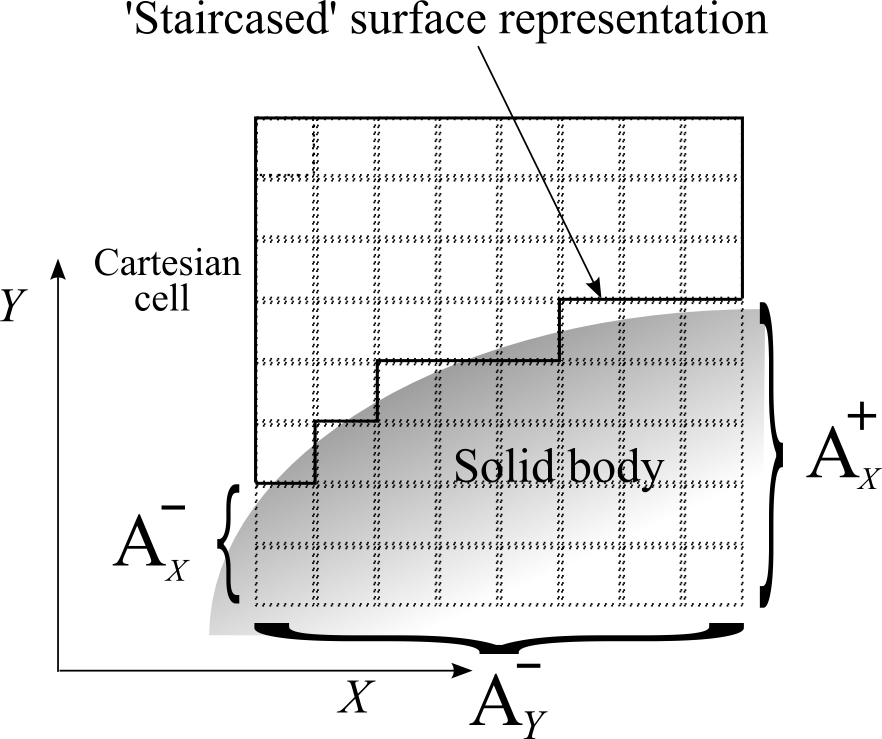
\includegraphics[width=5cm]{pics/VCE_staircase.jpg}
        }
        \subfigure[Planar surface]{
          \label{fig:VCE_way2}
          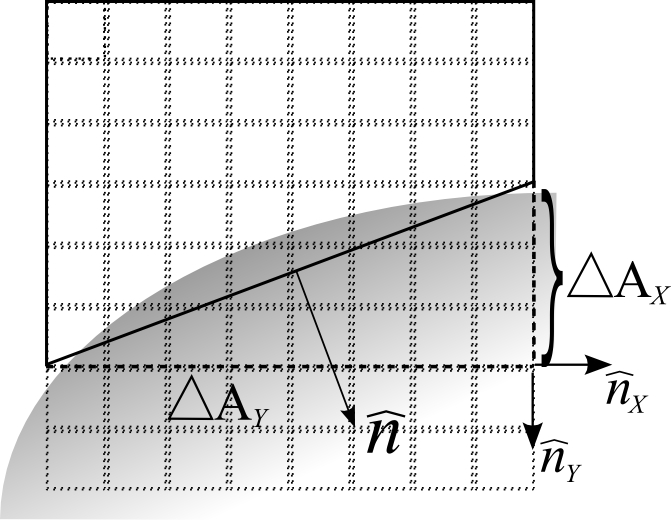
\includegraphics[width=5cm]{pics/VCE_smooth.jpg}
        }
        \label{fig:VCE}
        \caption{VCE method}
\end{figure}

\section{Octree domains}\label{sec:domain}

OctVCE implements isotropic subdivision of cubical cells as its \emph{h}-refinement procedure.  This approach lends itself
easily to an `octree' structure where a parent cell is refined to give 8 children (and similarly for the coarsening process),
as in fig~\ref{fig:octree_diag}.  Thus OctVCE starts with a \emph{root} cell which \textbf{corresponds to the numerical domain};
this root cell is then refined a certain number of \emph{levels} (the root is level 0) to give the initial mesh.

\begin{figure}[htp]
  \centering
  \label{fig:octree_diag}
  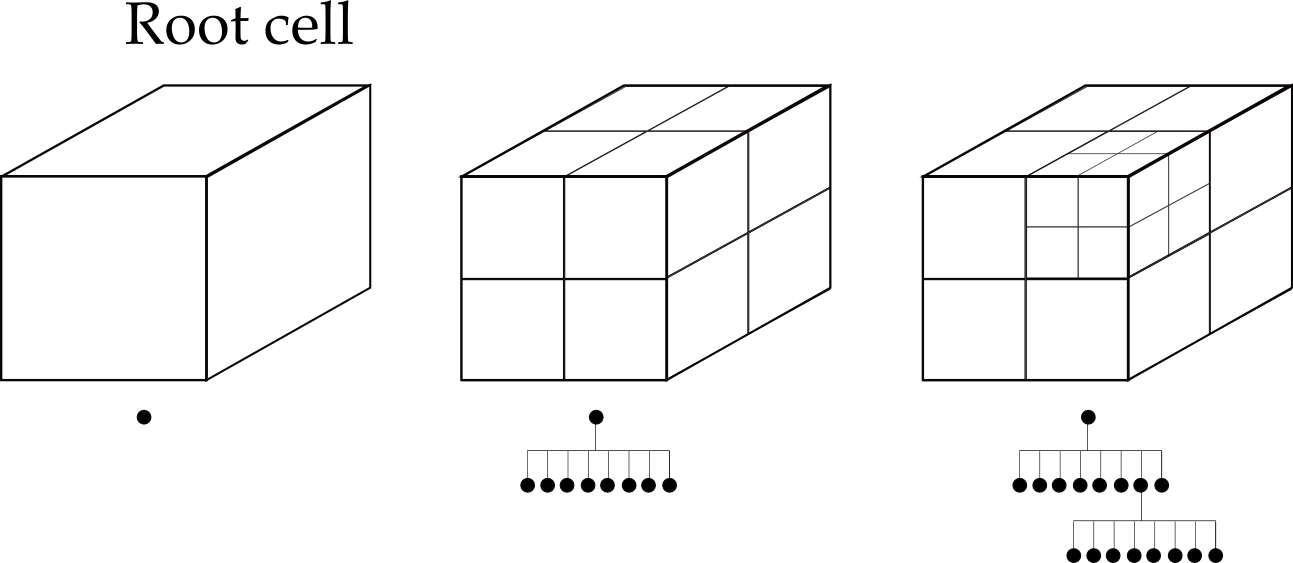
\includegraphics[width=7cm]{pics/octree_diag.jpg}
  \caption{Octree illustration}
\end{figure}

When the user enters the size and location of the root cell the numerical domain's extent is fully specified.  The 
root cell's dimensions are chosen to immerse the mesh appropriately within an environment of solid objects (whose locations
are usually known beforehand).  Whilst solid wall boundary conditions are implemented automatically by the cartesian cell method
by the presence of solid objects, the user is required to specify an appropriate \emph{domain boundary condition} for each
of the 6 faces of the root cell as they represent the borders of the numerical domain.             

\section{Initializing explosions}\label{sec:explo}

The initial explosion or `bomb' is represented by a volume or region of high pressure and density explosive gas (this approach is
also adopted by Timofeev et al \cite{Timofeev:au}).  These explosive gases can be modelled with the perfect gas, JWL \cite{Lee:ae}
or JWLB \cite{Baker:io} equation of state (described in further detail in $\mathsection$\ref{sec:JWLB}).  It has been found that 
matching the required total explosive energy is much more
important than the initial shape or density of the explosion volume.  

Usually cells at the explosion volume are refined to
the highest permissible level to track the developing blast wave accurately from the start.  This method of mapping the
bomb volume to a cartesian cell representation `staircases' the charge and thus will not produce very accurate solutions in the 
near-field when the actual charge shape is similarly not staircased.  See \cite{Rose:thesis} for a `remapping' technique between 1D spherical, 
2D axisymmetric and finally 3D solutions is employed that gives higher accuracy; the approach here is simpler
and should hopefully be adequate in the mid- to far-field.

OctVCE also supports a `detonation-like' finite-energy release scheme where the explosion volume is treated as a solid 
explosive i.e.\ all the cells within the explosion volume are not part of the computational domain. 
Ignition points are specified at locations within the explosive with
a `detonation' wave moving outward at constant velocity which `activates' the cells, initializing them to a specified high
pressure and density.  This not an actual detonation process, but is useful for more detailed modelling of non-uniform
blast in the near-field as the location of charge initiation can sometimes have an effect on both peak overpressure 
and impulse \cite{Anderson:ao}. 

\subsection{Initial conditions for JWL or JWLB equations of state}\label{sec:IC_advice}

As OctVCE cannot simulate an actual detonation process, one might ask to what pressures or densities the initial bomb
should be set.  Typically the density of the bomb $\rho_b$ chosen is the undetonated density $\rho_0$ (or loading density) of the 
explosive.  This 
is to get the correct initial mass and volume.  The initial JWL or JWLB explosive or chemical energy $E_0$ for the bomb is also 
assumed (this value is reported for various explosives in \cite{Lee:ae,Baker:im}).  The pressure is then calculated using
the equation of state i.e.\ $p = p\left(\rho_b,E_0\right)$.

The mapping of a bomb shape to the cartesian grid means that it will be difficult to match exactly the same volume occupied by 
the actual explosive.  Depending on the grid resolution, this can result in a considerable mismatch of initial explosive energy 
if the same explosive density $\rho_0$ and energy $E_0$ are used as the initial condition.  However, as will be seen in
$\mathsection$\ref{sec:smith_run} OctVCE can also conveniently output the total volume of cells representing the bomb volume $V_b$.  This 
information can be used to alter the initial explosion condition so that the initial explosive energy matches exactly the
actual energy.

For example, suppose exact matching of the the blast energy density $E_0$ (in J/kg) and bomb mass $m$ is desired.  The 
total blast energy is then $E_b = mE_0$.  The match is ensured by simply adjusting that $\rho_b = m/V_b$.  It is also possible to assume 
that the undetonated density $\rho_0$ in the JWL equation of state (eqn~\ref{eq:JWLB}) is equal to this value of $\rho_b$ instead of 
the figure reported in the literature.  

\section{The JWL and JWLB equations of state}\label{sec:JWLB}

It is useful to describe the actual JWL and JWLB equations of state here for later reference.  The JWLB equation of state is
\begin{equation}\label{eq:JWLB}
p = p\left(\rho, e \right) = \sum_{i = 1}^{n} A_{i}\left(1 - \frac{\lambda\left(\widetilde{v}\right)}{R_{i}\widetilde{v}}\right)e^{-R_{i}\widetilde{v}} + \frac{\lambda\left(\widetilde{v}\right) e}{v} + C\left(1 - \frac{\lambda\left(\widetilde{v}\right)}{\omega} \right){\widetilde{v}}^{-(\omega + 1)}
\end{equation}

where the Gr\"{u}neisen coefficient $\lambda$ given by 
\begin{equation}\label{eq:lambda}
\lambda\left(\widetilde{v}\right) = \sum_{i = 1}^{n}\left(A_{\lambda_{i}}\widetilde{v} + B_{\lambda_{i}} \right)e^{-R_{\lambda_{i}}\widetilde{v}} + \omega
\end{equation}

and $\widetilde{v} = v/v_0$.

$v = 1/\rho$ is the specific volume of explosion products whilst $\rho_0 = 1/v_0$ is the undetonated (loading) density of the 
solid explosive.  The constants $A_{i}$, $R_{i}$, $A_{\lambda_{i}}$, $B_{\lambda_{i}}$, $R_{\lambda_{i}}$, $C$, $\omega$ and $v_0$ can 
be found for various explosives in \cite{Baker:im}.  At most $n = 5$. Note that $A_i$ and $C$ are dimensional (in units of 
pressure), whilst $R_{i}$, $A_{\lambda_{i}}$, $B_{\lambda_{i}}$, $R_{\lambda_{i}}$
and $\omega$ are non-dimensional (thus $\lambda\left(\widetilde{v}\right)$ is also non-dimensional). 

Note that the JWL equation of state is basically the JWLB equation with  
$n = 2$, $C = 0$ and $\lambda = \omega$ (so with all $A_{\lambda_{i}}$ and $B_{\lambda_{i}}$ zero).  Constants for the JWL equation
are provided in \cite{Lee:ae}.

It is also important for later purposes to note the temperature-dependent form of these equations of 
state i.e.\ $p = p\left(\rho, T\right)$.  The temperature dependent form for the JWLB equation is quite lengthy but is
reported in \cite{Baker:io}.  However the JWL form is much simpler and can be written here as

\begin{equation}\label{eq:JWL_T}
  p = A_1e^{-R_1 \widetilde{v}} + A_2e^{-R_2 \widetilde{v}} + \omega \rho C_v T
\end{equation}

where $C_v$ is the specific heat at constant volume for the explosion products.

\chapter{Code compilation}\label{sec:code_compile}

OctVCE works best under a Unix or Linux system.  To compile OctVCE, both the \verb'Octvce3.5.'$\star$\verb'/' (where $\star$ is the 
subkernel version) and  \verb'Geomio/' directories are required.  The latest subkernel version as of April 2007 is \verb'4'.
These directories should be placed within the same level directory.  

The code is compiled using the \emph{makefile} in the \verb'Octvce3.5.'$\star$\verb'/unix/' directory.  
Near the top of the \emph{makefile} there are 3 variables which need to be set by the user.  Their function will be described 
below, along with some advice on how they can be set. 

\begin{enumerate}
\item \verb'CC' -- the compiler name e.g.\ \verb'icc' or \verb'pgcc' (an OpenMP compiler \cite{openmp:manual} is necessary for 
  parallel processing)
\item \verb'CFLAGS' -- the compiling options (which are compiler dependent) e.g.\ \verb'-O3'.

  \textbf{Note} -- at present a \verb'-static' flag (especially under the Intel compiler) is not recommended as it causes the code to 
  consume exorbitant system memory.  This author is still working on the cause for this (though this flag is not really necessary anyway).
\item \verb'OUT_DIR' -- where the executable \verb'octvce.exe' is placed.  

By default this is in \verb'Octvce3.5.'$\star$\verb'/tests/'
\end{enumerate}

In the past the author has typically compiled with the Intel compiler with flags like \verb'-O3', \verb'-openmp', \verb'-ipo'
and \verb'-ip'.  With the Portland compiler the flags were \verb'-O3', \verb'-mp', \verb'-fastsse' and \verb'-Mipa=fast'.

The other variables \verb'OV_SRC_DIR' and \verb'GM_SRC_DIR' need not be altered, as they are already set to where the source files
are located.  If it is absolutely necessary to move \verb'Geomio/' to some other location, both the \emph{makefile} variable
\verb'GM_SRC_DIR' and the header file locations in \verb'Octvce3.5.'$\star$\verb'/source/ov_kernel.h' need to be altered correspondingly.
After setting these variables appropriately just type \verb'make' and the executable should be produced.

\chapter{Setting up a simulation}\label{sec:sim_setup}

OctVCE requires several \emph{input files} for running simulations (assumed to be in the same directory that the executable \verb'octvce.exe' is located).  These files describe the solid geometry,
gas models, domain boundary conditions (see $\mathsection$\ref{sec:domain}), initial conditions, and other important
parameters like domain size, maximum refinement level, output frequency etc.  These input parameters will be
described below.  

\section{General simulation parameters input file}\label{sec:ov_par}

The general simulation parameters input file specifies to OctVCE such data as the root cell size and location, run parameters,
adaptation parameters, subcelling information and output frequency information.  It must be written \textbf{in exactly the same format}
as the template in fig~\ref{fig:ov.par} (a template can also be found in \verb'Octvce3.5.'$\star$\verb'/tests/ov.par').  
All words or spacings between lines in the file must follow the template exactly.  This lack of flexibility isn't as bad as it
seems as templates can be reused and modified repeatedly.  

A description of each input section (along with advice on what to input) will be described below.  Note that \textbf{any dimensional parameters are assumed to be in SI units} e.g.\ metres, seconds, pascals, joules, kilograms etc.  

\begin{enumerate}
\item \verb'Octree root spatial properties' 

\emph{Description} :-- Specifies location and size of the cubical root cell i.e.\ computational domain.

\emph{Parameters to input} :--
\begin{enumerate}
  \item \verb'Centroid location:' -- enter where in physical space the root cell should be centered
  \item \verb'Edge length scale:' -- enter the edge length of the root cell
\end{enumerate}

\item \verb'Run parameters' 

\emph{Description} :-- Some parameters on how the flow is solved numerically

\emph{Parameters to input} :--
\begin{enumerate}
  \item \verb'Type of flux solver:' -- options include \verb'AUSM', \verb'AUSMDV', \verb'EFM', \verb'ADAPTIVE'

    The \verb'ADAPTIVE' option uses a combined solver where EFM is used at shocks and AUSMDV elsewhere, which is handy
    for eliminating odd-even decopuling issues \cite{Quirk:ac2}.
        
  \item \verb'Use multiple limiters?' -- enter in \verb'y' or \verb'n'

    Under the present methodology the extreme initial conditions at an explosion's beginning can 
    sometimes cause the higher-order reconstruction scheme to fail (especially if the JWL or JWLB equation is used).  Using a single 
    global limiter can prevent this instability, though multiple limiters give a more accurate solution.  More discussion on
    the failure of OctVCE's flow solver is also found in $\mathsection$\ref{sec:sim_run}.

  \item \verb6Global timestep (set to 0 if don't want it fixed):6 -- usually this is set to 0 to allow for varying timesteps.

  \item \verb'Max CFL (must be between 0 and 1):' -- enter in the \emph{maximum allowable} CFL number.  Usually this is set to 0.5.  
    Strong explosions may require such small timesteps initially that the CFL may
    need to be quite low at the beginning of a simulation.  Eventually this CFL number ramps back up to the maximum allowable
    value.

  \item \verb6Finish time (choose one and make the other '0')6 -- simulation finishes either when a set number of timesteps is
    exceeded or flow time exceeded.  If finish time is measured by timesteps/flow time, a \verb'0' must be put in
    the other field.
\end{enumerate}

\item \verb'Parallel processing'

\emph{Parameter to input} :--

\verb'Adapt in parallel?' -- enter in \verb'y' or \verb'n'

Usually this is \verb'y'.  If parallel processing isn't employed, this line is ignored.  
OctVCE can parallelize the adaptation procedure, which generally gives faster code for
simulations involving many cells.  But sometimes the extra work in forking and joining threads might be too time-intensive
for small simulations.

\item \verb'Adaptation parameters'

\emph{Description} :-- Specifies adaptation option, and thresholds for refinement and coarsening around flow features like 
shocks or contact discontinuities

\emph{Parameters to input} :--
\begin{enumerate}
  \item \verb6Adapt every how many time steps (enter '0' for no adaptation):6 -- if adaptation is desired, `5' is a recommended number, 
    else `0' for no adaptation 
  \item \verb'Type of error indicator:' -- options are \verb'1', \verb'2', \verb'3'

    Please consult \cite{Tang:tm} for further documentation regarding adaptation indicators.  Indicator \verb'1' corresponds
    to the shock-detection scheme based on velocity gradients.  Indicator \verb'2' uses density differences (good for
    detecting contact discontinuities).  Indicator \verb'3' simply means indicators \verb'1' and \verb'2' being used together.

    \item \verb'If error indicator type is 1 or 3 - compression threshold:' -- a value from 0.05 to even 0.005 is acceptable.  The smaller 
      the number, the greater the chance that weak compressions (not shocks) will also be refined about.

    \item \verb'If error indicator type is 2 or 3 ...'
      \begin{enumerate}
	\item \verb'Refinement threshold:' -- the user must experiment with this, but 0.3 seems like a good starting figure for many
	  calculations.  If flow features are quite weak, this number may need to be reduced.
	\item \verb'Coarsening threshold:' -- the user must experiment with this, but it must be smaller than the 
	  refinement threshold.  0.1 seems like a good starting figure, though the author has used values as low as 0.01.  The
	  lower the value, the better chance the weaker features will still be refined about.
	\item \verb'Noise filter value:' -- this can vary between 0.001 to 0.1.  The larger the value, the less chance for refinement
	  around compressions.  The user must experiment with this.
      \end{enumerate}
\end{enumerate}

\item \verb'Octree refinement parameters'

\emph{Description} :-- Specifies subdivision of root cell to form initial grid, minimum and maximum refinement levels when adaptation
is used.  

\textbf{Note} -- the root cell is at level 0; if it is refined $n$ times the leaf cells will be at level $n$.

\emph{Parameters to input} :--
\begin{enumerate}
  \item \verb'No. times to refine root initially:' -- this refines the root cell \emph{uniformly} to create the initial grid (which
    would also be the final grid if adaptation isn't employed).  However if any cells are known
    to be `solid' i.e.\ completely immersed in a body, it won't be refined any further.  Usually the initial grid can be fairly 
    coarse, so this number is typically smaller than 8.
  \item \verb'Max refinement level:' -- this obviously has to be a higher level than the initial grid level.  The highest level
    of refinement used thus far by the author has been 11.
  \item \verb'Min refinement level:' -- usually this is the same as the initial grid level.
  \item \verb'Min intersect refinement level:' -- specifies the minimum level that \emph{partially obstructed} cells should be at.
    All cells with objects cutting through their \emph{volumes} will be refined to this level.  Sometimes handy when higher resolution
    is required at surfaces, but generally this has been set to the initial grid level.
  \item \verb'Level of cell IC intersection:' -- specifies the level that cells intersecting the initial bomb volume (see 
    $\mathsection$\ref{sec:explo}) should be at.  Usually this is set to the maximum refinement level.
\end{enumerate}

\item \verb'Geometry engine parameters'

\emph{Description} :-- Provides data for the geometry engine to complete its process of approximating surfaces with VCE in 
obstructed cells  

\emph{Parameters to input} :--
\begin{enumerate}
  \item \verb'Interrogate geometry engine only after what level:' -- specifies for what cell levels the actual point-in-polyhedron
    queries will be performed.  A higher figure means more computation (but more accuracy).  It's generally set to the same level as 
    the initial grid level.  But if the initial grid level is very high (say $\ge$ level 7), a lower number will give substantially
    faster gridding time.
  \item \verb'No. area subcells along edge (must be even):' -- the number of subcells $ns_f$ \emph{along} a single cell face 
    edge.  The total number of subcells on one cell face is thus ${ns_f}^2$.  The higher the number, the
    more accurate the surface representation.  Usually between 20 and 64 (but for 2D simulations, see $\mathsection$\ref{sec:2D}).
  \item \verb'No. volume subcells along edge (must be even):' -- the number of subcells $ns_v$ along a cell volume edge. The total 
    number of volume subcells is thus ${ns_f}^3$.  A number of about 10 to 16 should be sufficient.
  \item \verb6Wall representation ('0' for staircased, '1' for smoothed):6 -- as written, only \verb'0' or \verb'1' can be entered.
    See $\mathsection$\ref{sec:VCE} for explanation.  Generally a smooth wall (option \verb'1') is preferrable.
\end{enumerate}

\item \verb'Visualization'

\emph{Description} :-- Specifies what data to output and how often 

\emph{Parameters to input} :--
\begin{enumerate}
  \item \verb'Write flow soln of only intersected cells?' -- options are \verb'y' or \verb'n'.

    Generally \verb'n' is entered as the whole flowfield is desired.  If \verb'y' is used then only the output from cells
    intersected or flush with solid surfaces will be given (which gives a much smaller solution file).

  \item \verb6Write data frequency (choose one and make the other '0')6 -- usage is the same as with the finish time (see above).
    Either output every some number of timesteps or at a specified time interval.  If write data frequency measured by timesteps/flow time,
    a \verb'0' must be put in the other field.

    The solution files will be in the VTK XML format and have a \verb'.vtu' and/or \verb'.pvtu' extension.  
    See $\mathsection$\ref{sec:post_proc} for further information.

  \item \verb'Base solution file name:' -- enter in a name for the solution files.  Other information e.g.\ the timestep where
    the file is output and finally the \verb'.vtu' extension will be appended to this.
\end{enumerate}

\item \verb'History files'

\emph{Description} :-- Specifies at which locations the pressure history should be recorded.  See $\mathsection$\ref{sec:p_trace_file}
for further information on the output format of the pressure traces. 

\emph{Parameters to input} :--
\begin{enumerate}
  \item \verb'No. history locations:' -- how many pressure traces are desired?  If this is 0, all further lines will be ignored.
  \item \verb'Dump history locations every how many time steps:' -- how often should the pressure at a point be recorded.  Typically recording every 2 to 5 timesteps is enough.
  \item \verb'Base history file name:' -- enter in a name for the trace recording.  Other information e.g\ trace location is appended.
\end{enumerate}

\item \verb'History locations'

\emph{Parameters to input} :-- At each line enter in the gauge location where the pressure trace is recorded.  Must be a 3D point. 

\end{enumerate}

\begin{figure}[htp]
\centering
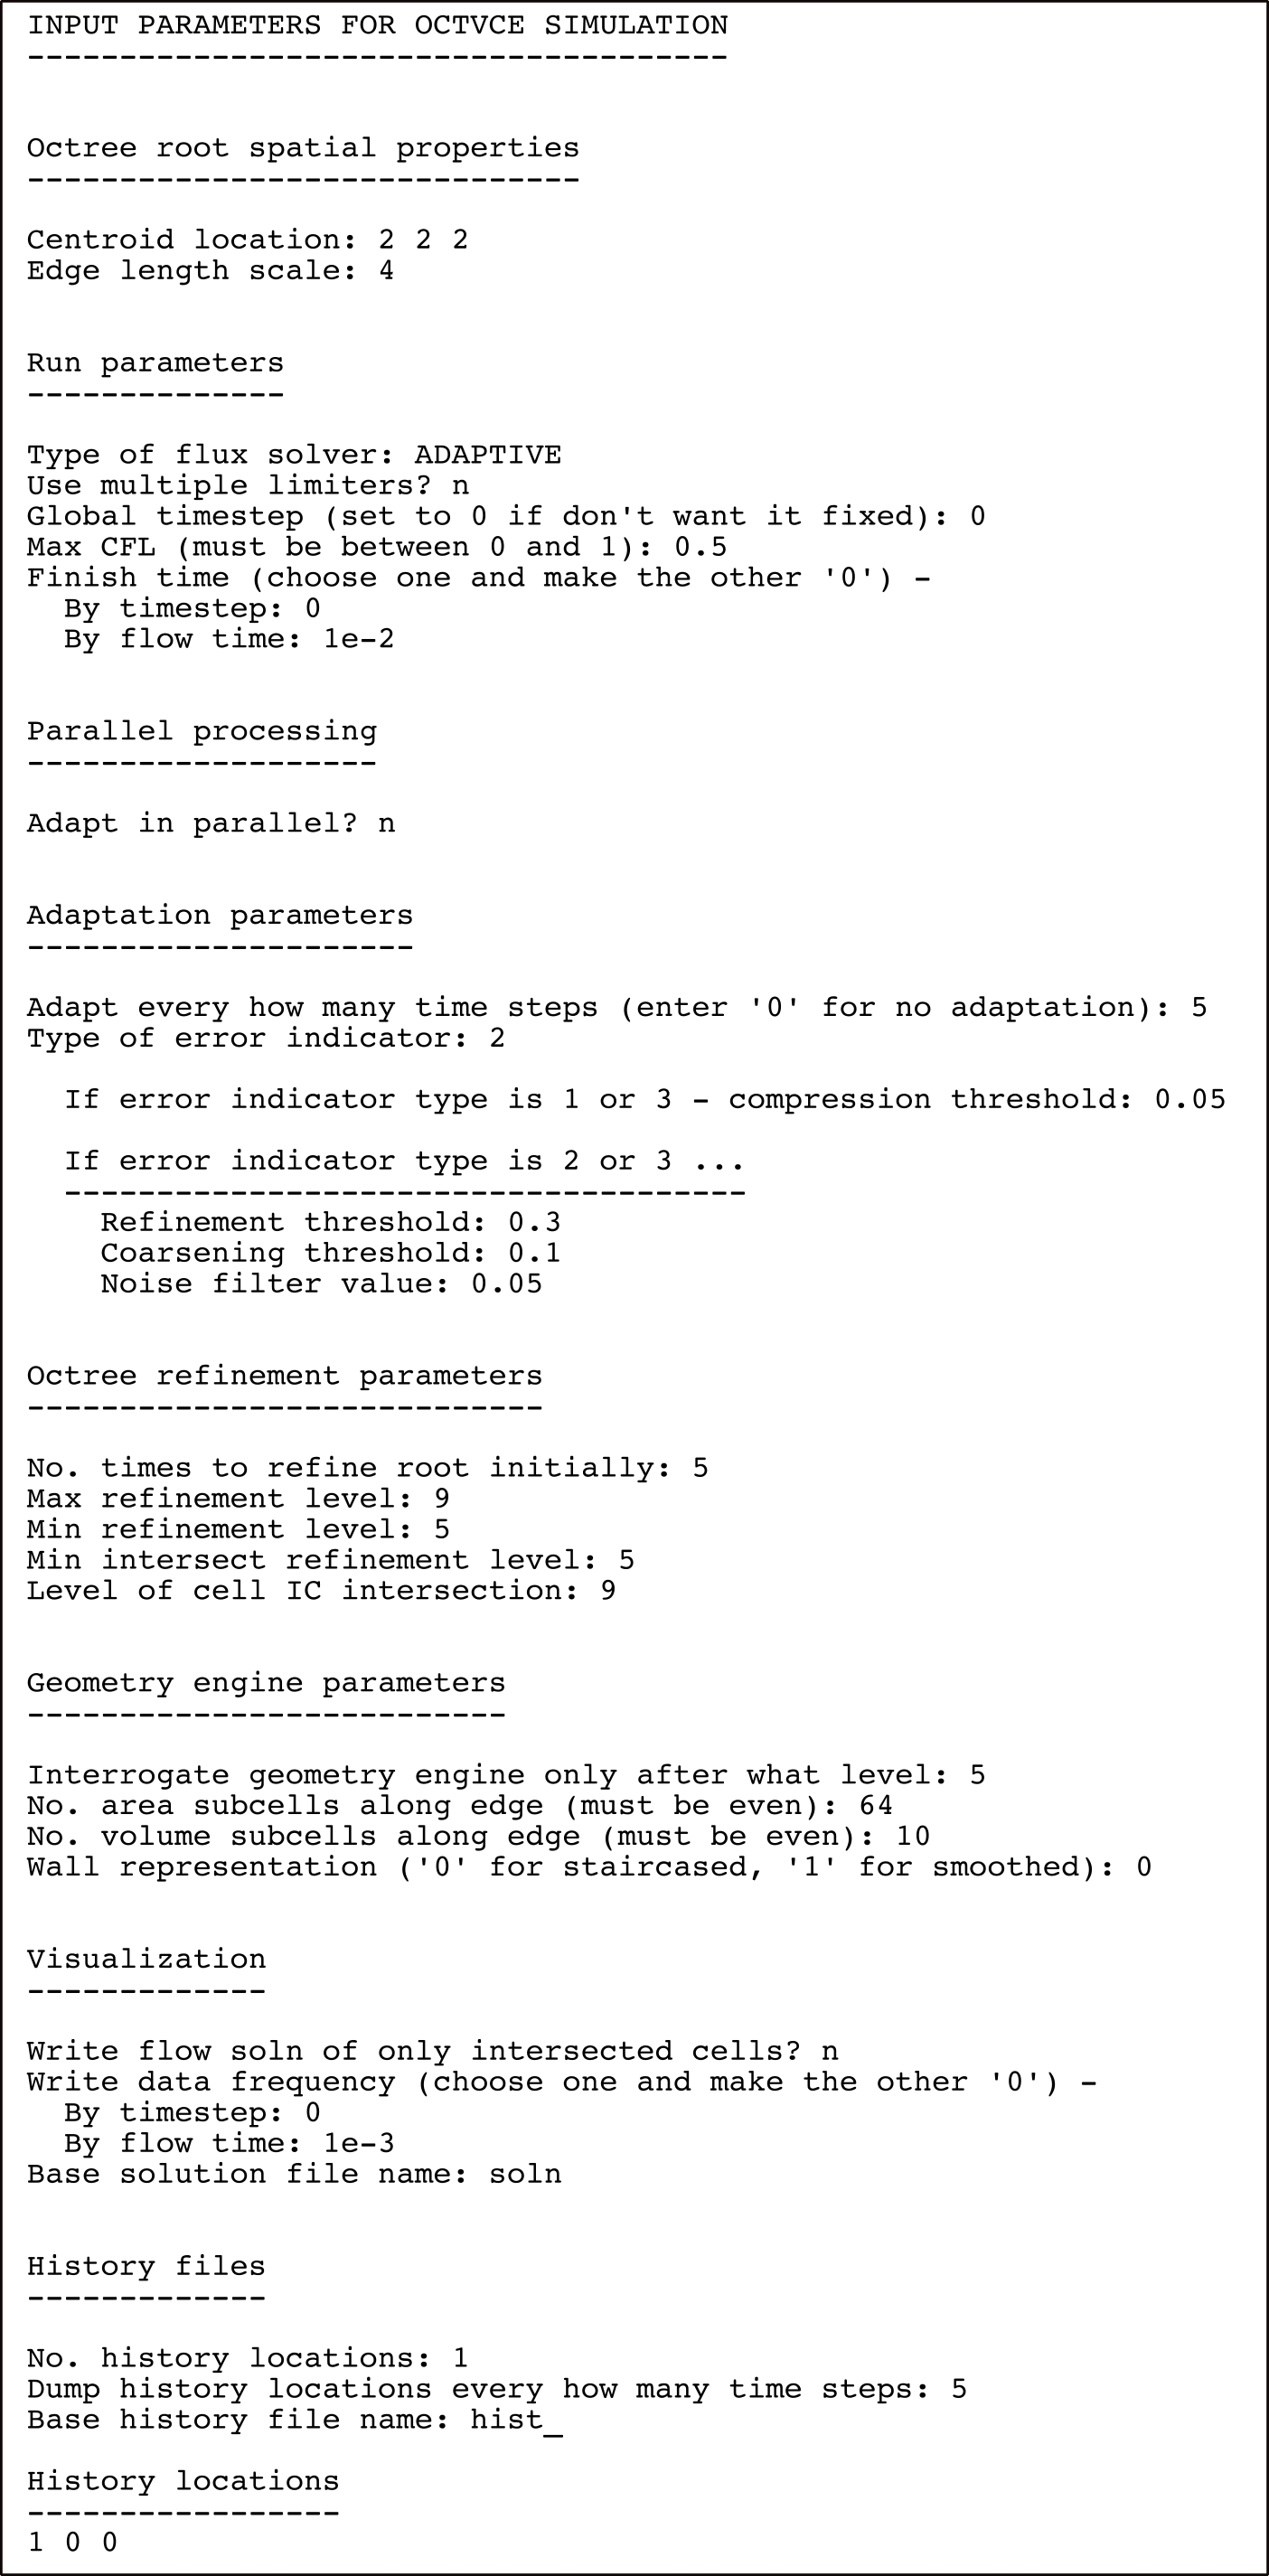
\includegraphics[width=11cm]{pics/ov_par_template.jpg}
\label{fig:ov.par}
\caption{General parameters file}
\end{figure}

\pagebreak

\section{Solid geometry definition}\label{sec:geom}

Each solid object in the computational domain must be 3D object and defined with the VTK XML version 4.2+ ASCII file 
format \cite{book:vtkmanual} definition\footnote{Or see www.vtk.org/pdf/file-formats.pdf} (commonly with a \verb'.vtp' 
extension).  However it is not necessary for VTK to be installed on the system as OctVCE contains its own VTK file parser.  

It is important all these objects are `watertight' i.e.\ no `holes' which may confound
the geometry engine, and that face definitions are defined in \emph{counterclockwise} fashion (using the right hand rule) so that
the surface normal points \emph{outward} from the surface.  

For example, fig~\ref{fig:vtp_cube} is a VTK file describing a unit cube (centered at $\left(0.5, 0.5, 0.5\right)$).  The     
\verb'<Polys>' dataset describes how the cube's verticies are joined to make the individual faces.  Note that the connectivity
data joins the verticies in the required counterclockwise order.  Only the \verb'Points', \verb'connectivity' and \verb'offsets'
data arrays are required to fully define a solid body.

\begin{figure}[htp]
\centering
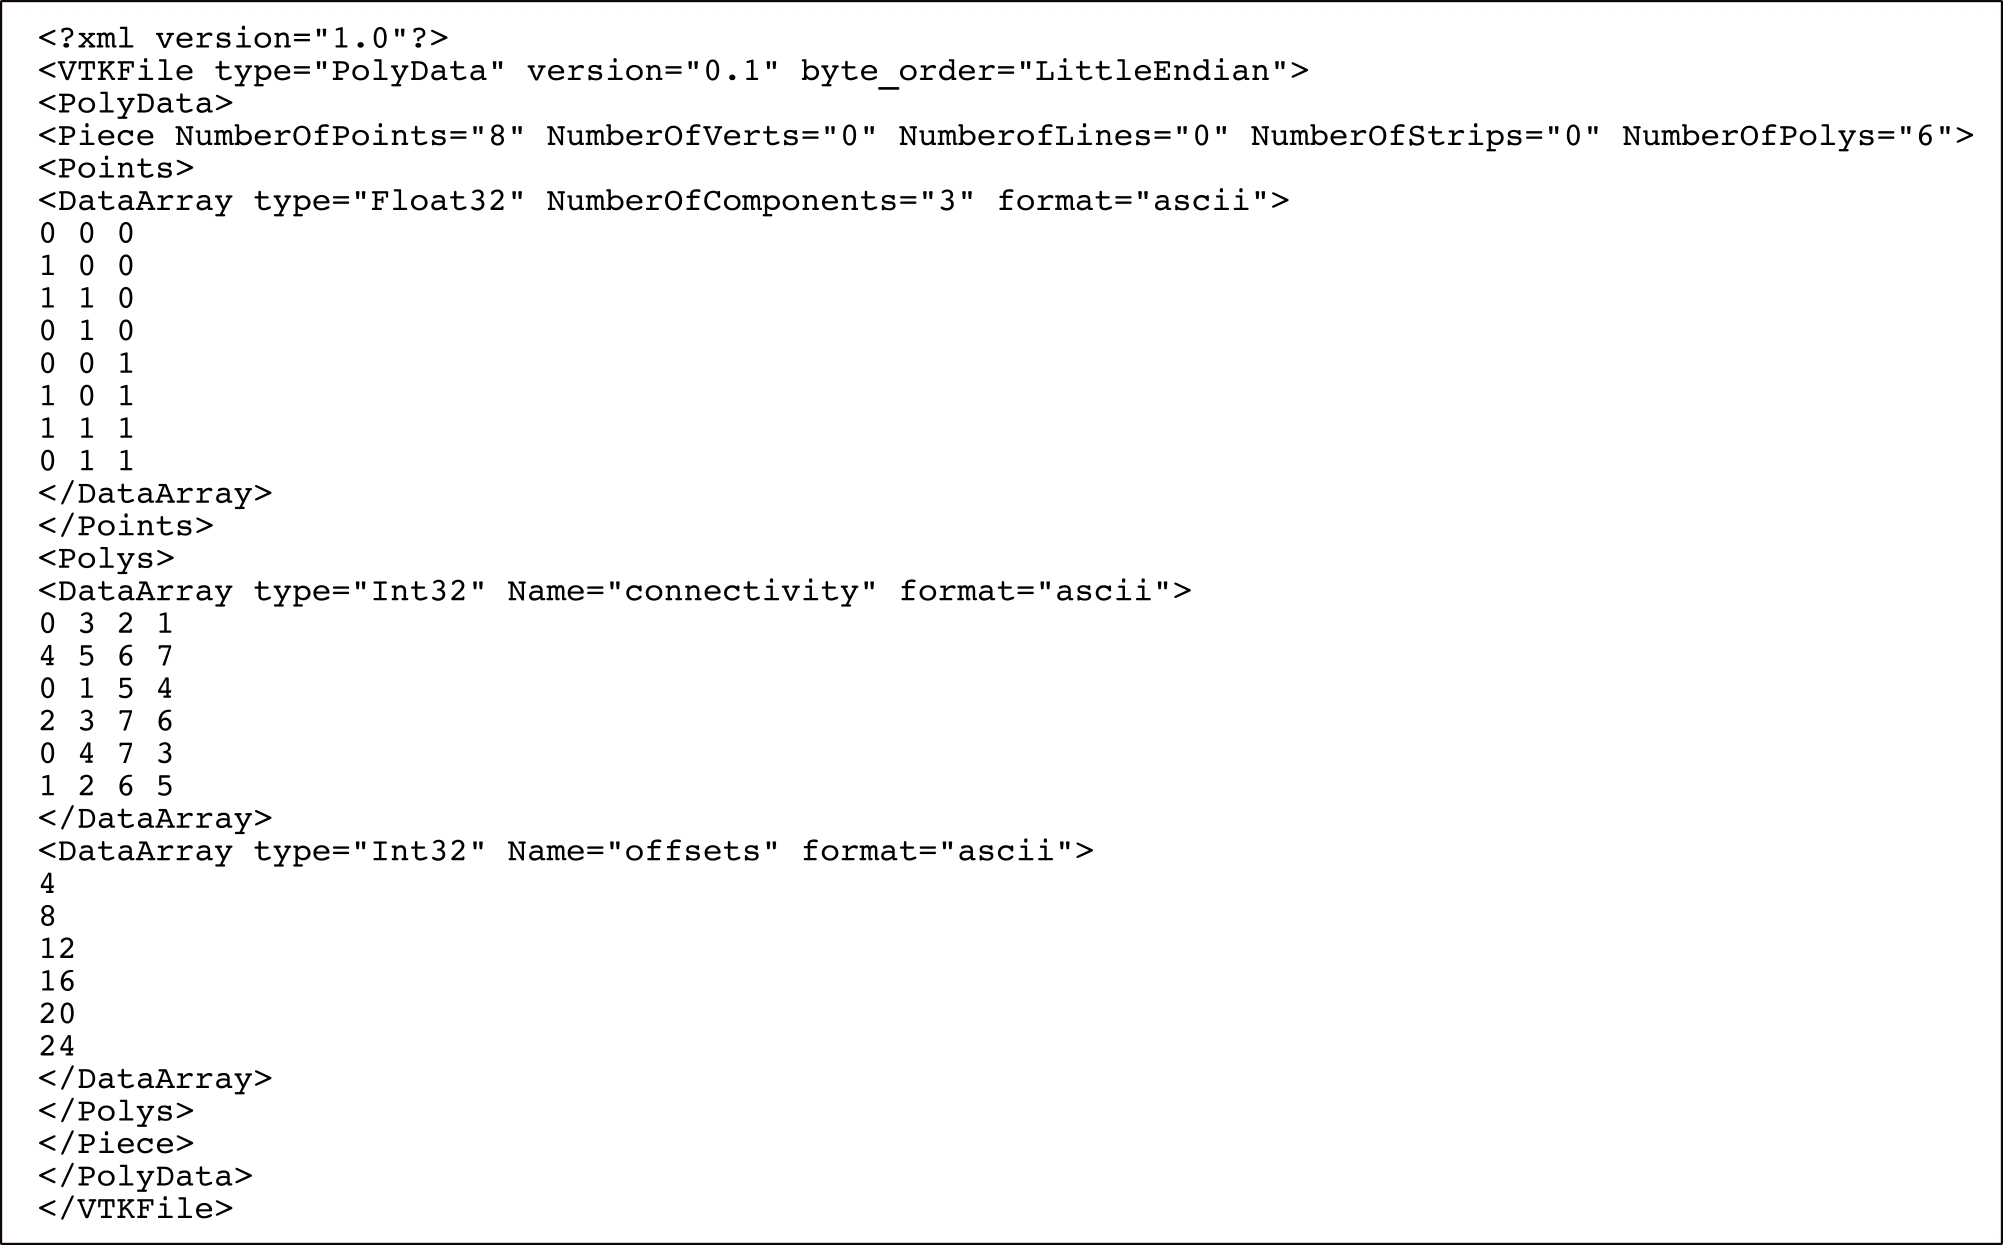
\includegraphics[width=17cm]{pics/VTP_cube_file.jpg}
\caption{Example VTP file of a cube}
\label{fig:vtp_cube}
\end{figure}

With a each solid object described by its own VTK file, the collection of solid objects is then placed in a 
`parallel' VTK file (with a \verb'.pvtp' extension) to describe the physical \emph{environment} of all objects.
Even if there is only 1 body it must be still entered into this file.  
An example parallel VTK file where 3 solid objects exist in the environment is provided in fig~\ref{fig:XML_eg}.

\begin{figure}[htp]
\centering
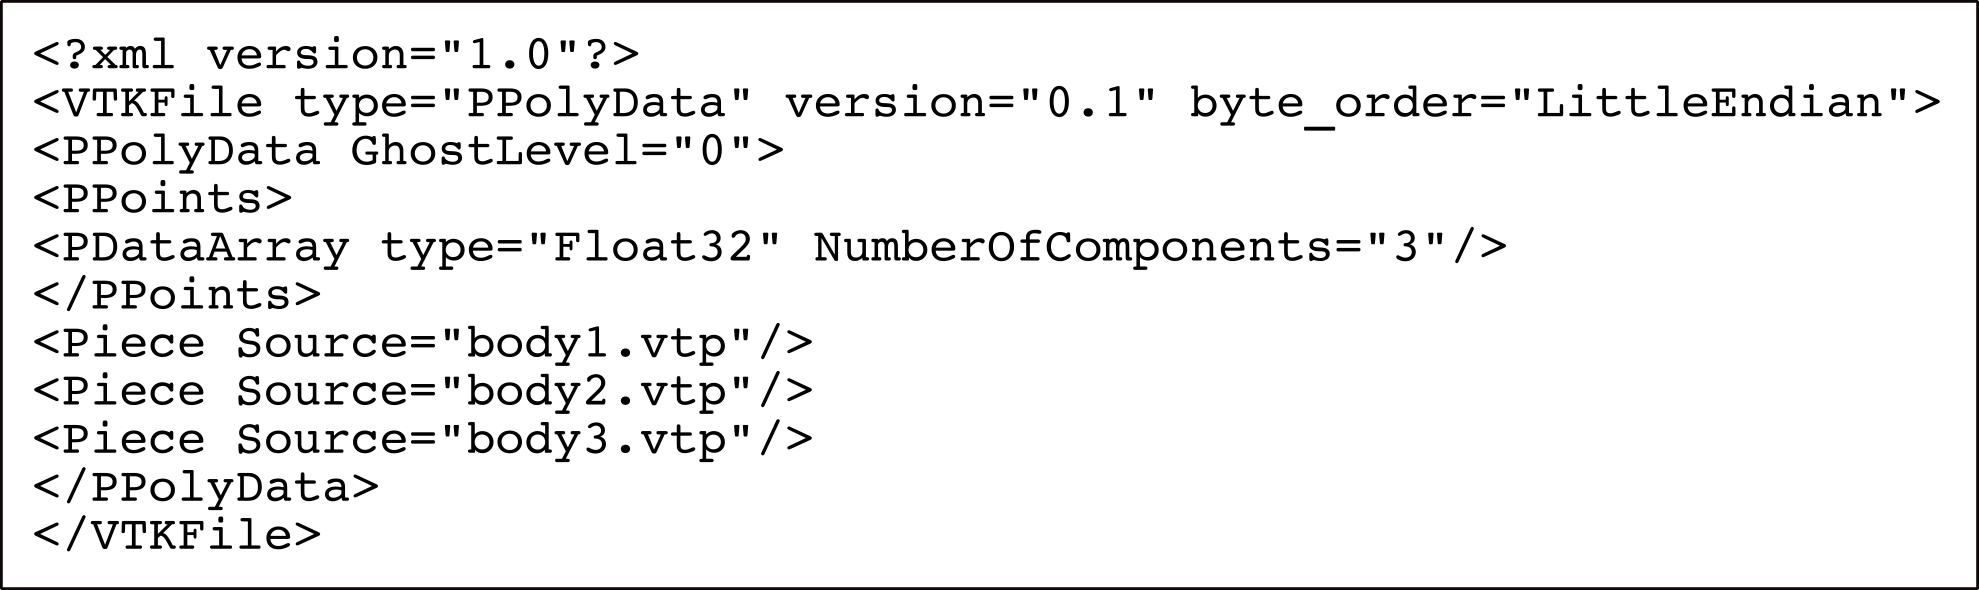
\includegraphics[width=14cm]{pics/PVTP_file.jpg}
\caption{Example PVTP environment definition}
\label{fig:XML_eg}
\end{figure}
\newpage
\subsection{A note on flushed surfaces}\label{sec:grid_flush}

In many situations there could exist solid bodies which are exactly flush with a grid line/plane e.g.\ in creating
a solid domain boundary (as in fig~\ref{fig:boundary_wall}).  This can sometimes present a problem of geometric tolerance
as OctVCE's geometry engine may on occasion compute the cell faces flush with the solid surfaces as unobstructed still.

\begin{figure}[htp]
\centering
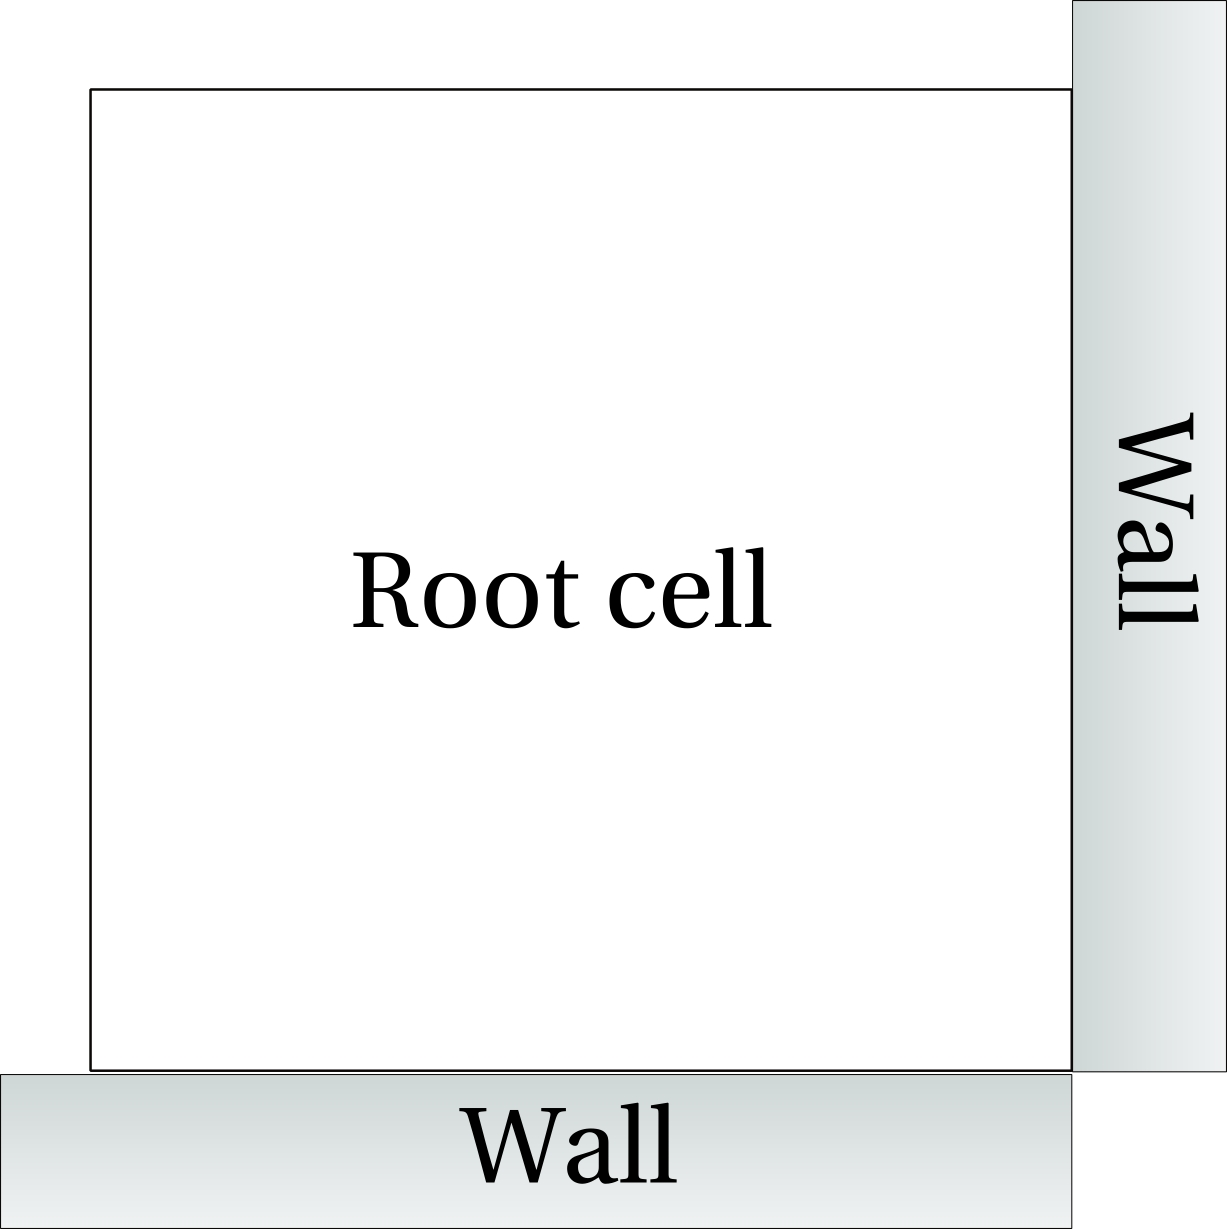
\includegraphics[width=3cm]{pics/flush_wall.jpg}
\caption{Boundary-aligned wall}
\label{fig:boundary_wall}
\end{figure}

The easiest solution is to have a small overlap between cells and the solid surfaces.  Two ways to do this are -- 
\begin{enumerate}
\item Modify the body VTK file so that the solid surface overlaps very slightly with the cell surface (increasing or
decreasing a dimension by $10^{-10}$ is enough)
\item Very slightly increase/decrease the root cell's edge (i.e.\ domain's) length to cause this overlap (again an increase of
$10^{-10}$ should be sufficient)
\end{enumerate}

\section{IC input file}\label{sec:ov_IC}

The initial condition input file specifies to OctVCE what the initial conditions in the computational domain should be.
When modelling explosions, OctVCE requires 2 initial conditions -- (a) the initial flow state for the ambient (commonly 
atmospheric) gas, and (b) the conditions for the initial explosion products (recall $\mathsection$\ref{sec:explo}).  

As with $\mathsection$\ref{sec:ov_par}, this file must be written in \textbf{exactly the same format} as the 
template in fig~\ref{fig:ov_IC.par} (a template can also be found in \verb'Octvce3.5.'$\star$\verb'/tests/ov_IC.par').
Note that \textbf{any dimensional parameters are assumed to be in SI units}.  A description of this file will be given below.

\begin{enumerate}
\item \verb'Ambient conditions' -- initial conditions for the ambient gas

\emph{Parameters to input} :--
\begin{enumerate}
  \item \verb'Pressure:' -- enter the pressure (in Pa) for the ambient gas (typically atmospheric conditions)
  \item \verb'Density:' -- enter the density (in $kg/m^3$) for the ambient gas (typically atmospheric conditions)
  \item \verb'U:' -- enter in the initial velocity (in $m/s$) along the $x$ axis 
  \item \verb'V:' -- enter in the initial velocity (in $m/s$) along the $y$ axis 
  \item \verb'W:' -- enter in the initial velocity (in $m/s$) along the $z$ axis 
\end{enumerate}

\item \verb'Products conditions' -- initial conditions for the explosive products gas

\textbf{Note} -- this whole section can be omitted if only ambient conditions are needed e.g.\ solving steady
state flow over a wedge where the initial conditions are the constant freestream conditions.

\emph{Parameters to input} :--
\begin{enumerate}
  \item \verb'Pressure:' -- enter the pressure (in Pa) for the initial explosion volume.  If the JWL/JWLB equation is 
    used see $\mathsection$\ref{sec:IC_advice} for an idea of what pressure to use.
  \item \verb'Density:' -- enter the density (in $kg/m^3$) for the initial explosion volume (see $\mathsection$\ref{sec:IC_advice}
    if the JWL/JWLB equation is used)
  \item \verb'U:' -- enter in the initial velocity along the $x$ axis (for high explosive modelling, is typically 0)
  \item \verb'V:' -- enter in the initial velocity along the $y$ axis (for high explosive modelling, is typically 0)
  \item \verb'W:' -- enter in the initial velocity along the $z$ axis (for high explosive modelling, is typically 0)
  \item \verb'File:' -- the name of the file describing the initial bomb geometry in the computational domain.

    The file is assumed to be in the same directory as the executable \verb'octvce.exe'.  It is exactly in the same
    format as those \verb'.vtp' files describing individual solid objects as discussed in $\mathsection$\ref{sec:geom}. 
\end{enumerate}
\end{enumerate}

\begin{figure}[htp]
\centering
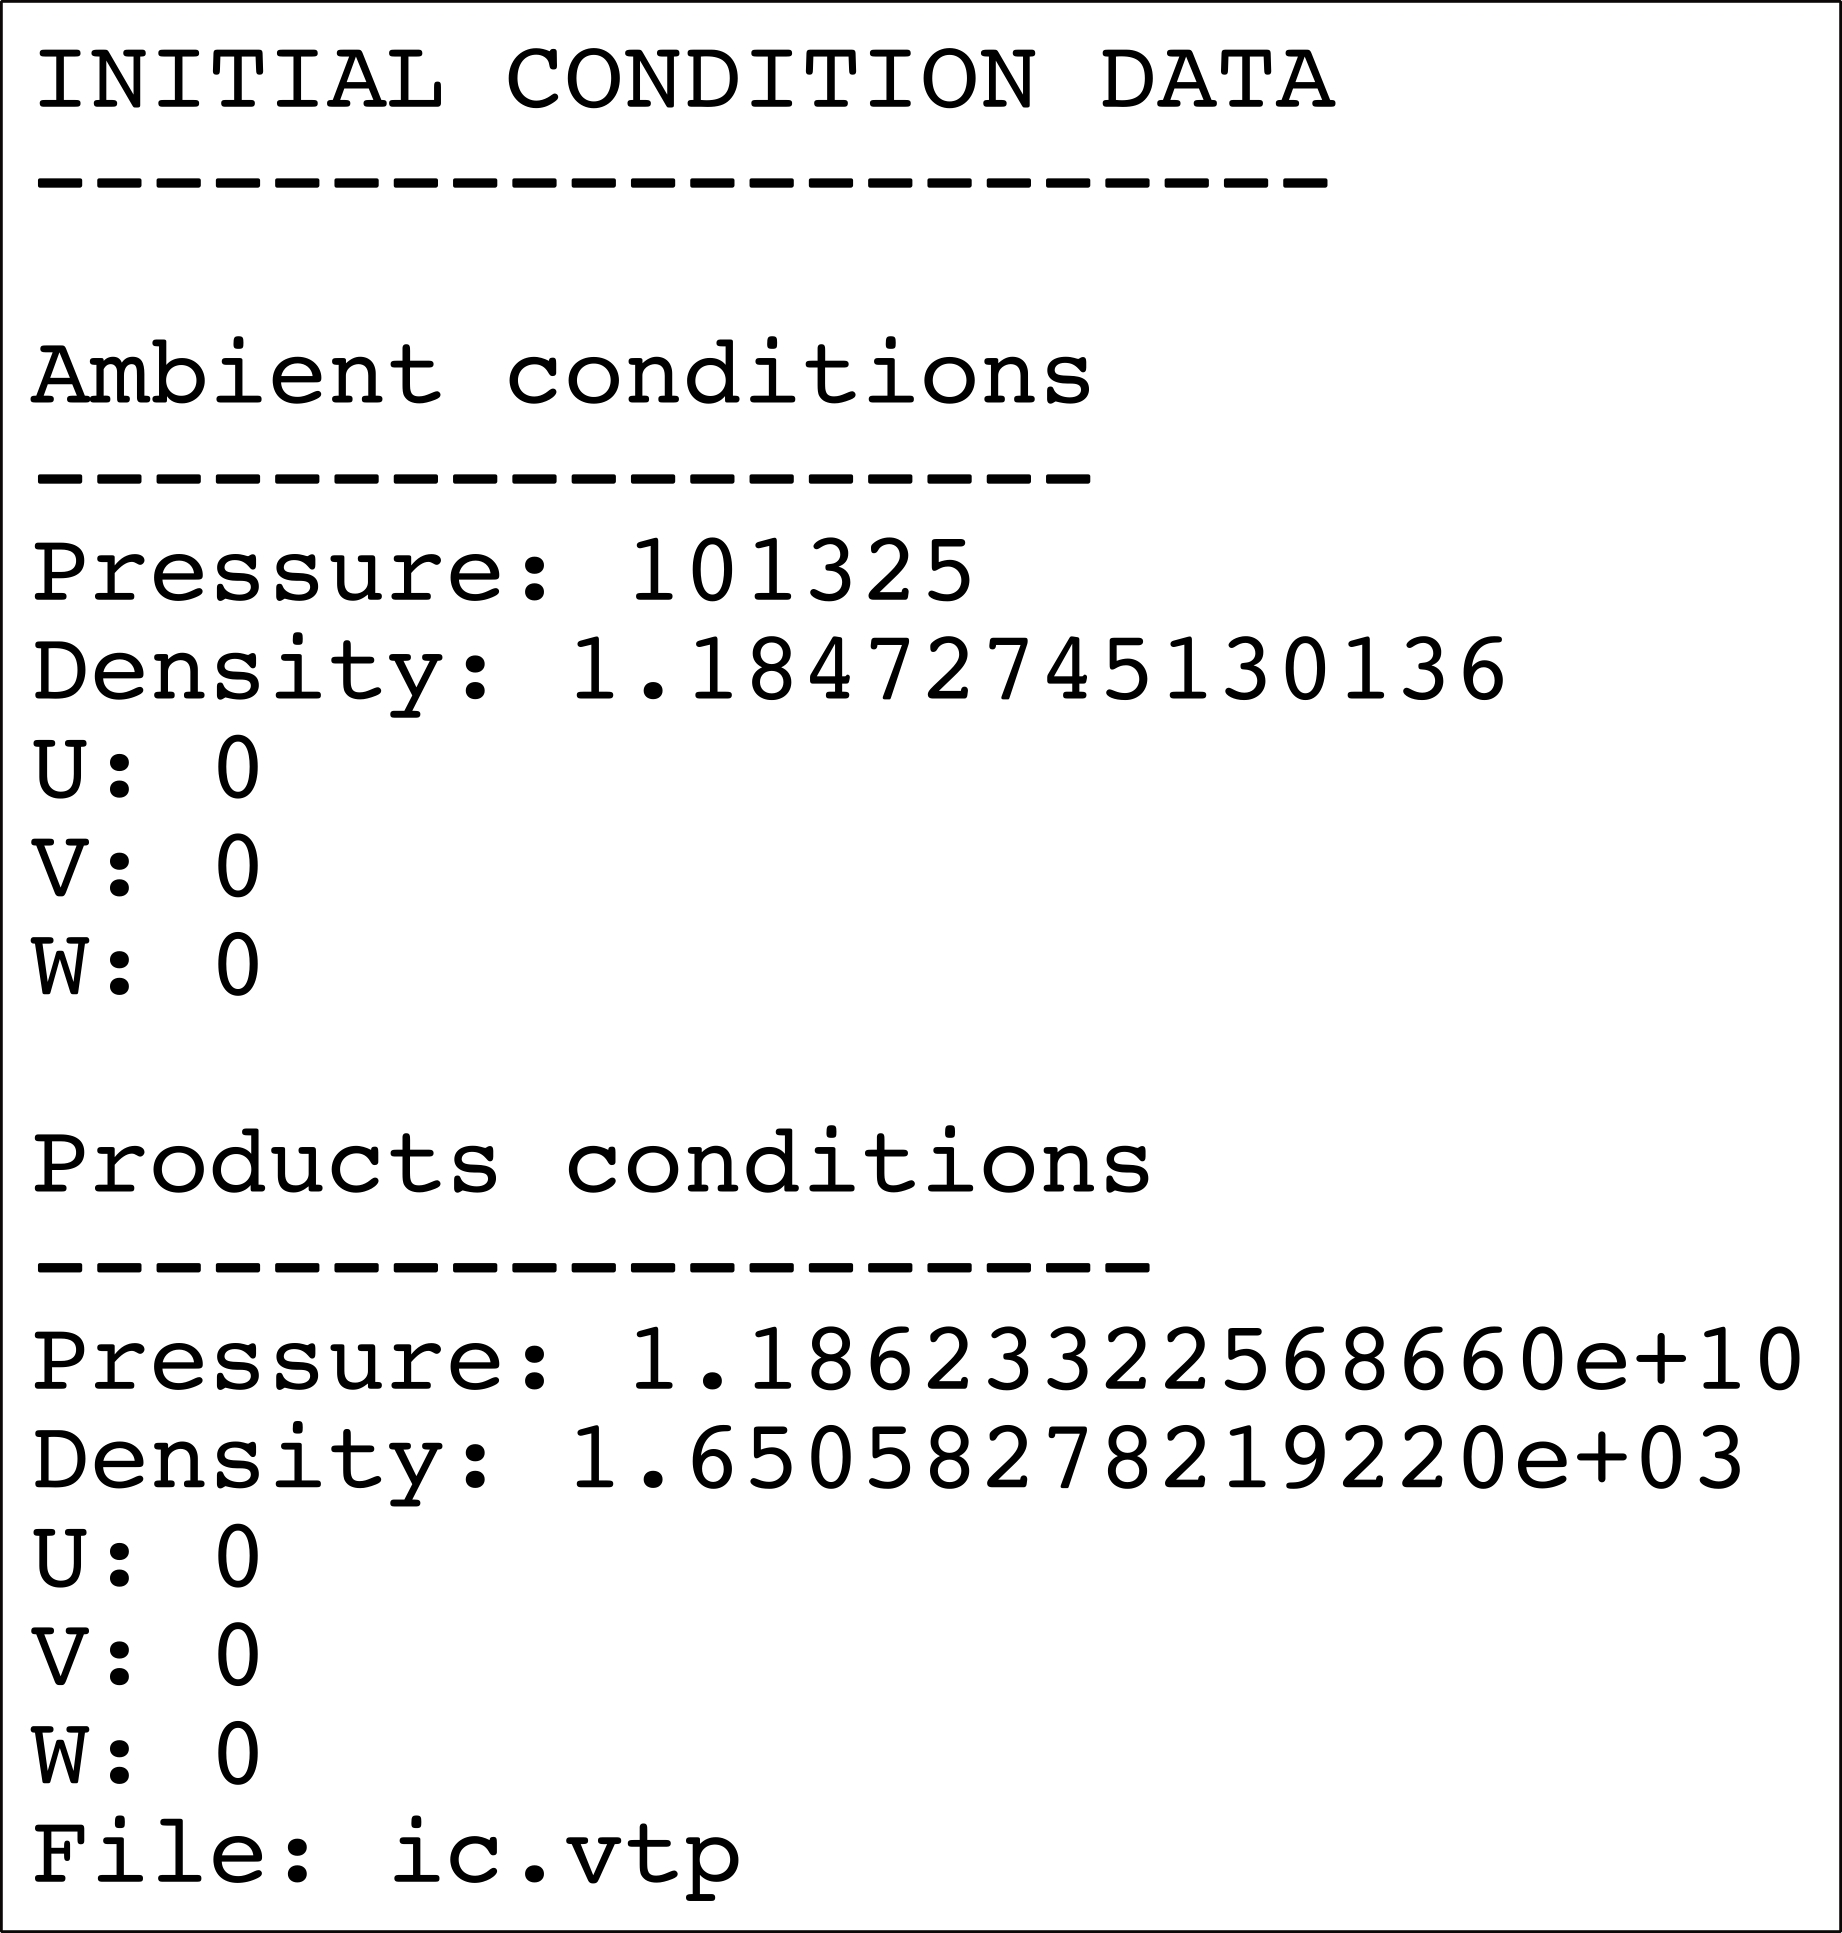
\includegraphics[width=5cm]{pics/ov_IC_template.jpg}
\caption{Initial condition file (2 species)}
\label{fig:ov_IC.par}
\end{figure}

\pagebreak

\section{Gas model input file}\label{sec:ov_gas}

The gas model input file specifies to OctVCE what gas models to use for the ambient and explosive products gases (see
$\mathsection$\ref{sec:ov_IC}).  The ambient gas is always modelled with ideal gas equation of state $p = \rho e\left(\gamma-1\right)$,
but the explosive products can be modelled with the ideal gas, JWL or JWLB equations of state (see $\mathsection$\ref{sec:JWLB}).

As with $\mathsection$\ref{sec:ov_IC}, this file must be written 
in \textbf{exactly the same format} as the template in fig~\ref{fig:ov_gas.par} (a template can also be found 
in \verb'Octvce3.5.'$\star$\verb'/tests/ov_gas.par').  Note that \textbf{any dimensional parameters are assumed to be in SI units}.  A 
description of this file (along with some advice on what to input) will be given below.

\begin{enumerate}
  \item \verb'No. species:' -- options are \verb'1', \verb'2'

    The number of gas species in the simulation.  Typically for high explosive modelling it's 2 (the ambient and explosive products
    gases).

  \item \verb'Ambient gas Cv:' -- enter in the specific heat at constant volume for the ambient gas

  \item \verb'Ambient gas gamma:' -- enter in the ratio of specific heats for the ambient gas

  \textbf{Note} -- if only 1 species (i.e.\ the ambient gas) is used all following lines are ignored as this information is sufficient

  \item \verb'EOS type for products:' -- options are \verb'Ideal', \verb'JWLB'

    Recall from $\mathsection$\ref{sec:JWLB} that the JWL equation of state is a simplified form of the JWLB one 

  \item \verb'Products gas Cv:' -- enter in the constant specific heat at constant volume for the explosive products

    Usually $C_v$ is calculated so as to match a known pressure and temperature condition.  For example, if the
    JWL equation of state is used, eqn~\ref{eq:JWL_T}
    can be used to back-calculate $C_v$ if the initial temperature and pressure of the explosion is known (recall 
    $\mathsection$\ref{sec:explo} and $\mathsection$\ref{sec:ov_IC}).  Mader \cite{Mader:book} provides initial detonation
    temperatures for some explosives.

  \item \verb'Products gas gamma:' -- enter in the ratio of specific heats of the explosion products (if the ideal gas equation
    of state is used)

  \item \verb'If EOS is JWLB - want to treat low products density as air?' -- options are \verb'y' or \verb'n'

    To save computation time, regions where density of the explosive products is very low can be just regarded as air if \verb'y' is
    selected.  This is usually the preferred option.

  \item \verb'If EOS is JWLB - EOS coefficients are' -- enter in all JWL/JWLB constants in the following lines

    Using eqn~\ref{eq:JWLB} as reference, \verb'A1' for example corresponds to $A_1$, \verb'R1' to $R_1$, \verb'AL1' to $A_{\lambda_1}$,
    \verb'BL1' to $B_{\lambda_1}$, \verb'RL1' to $R_{\lambda_1}$, \verb'OMEGA' is $\omega$ and \verb'v0' is $1/\rho_0$.
    Recall from $\mathsection$\ref{sec:JWLB} that $A_i$ and $C$ are dimensional and here are in units of pascals, and $v_0$ is
    in units of $m^3/kg$.
    
    The example in fig~\ref{fig:ov_gas.par} is the JWL equation of state where appropriately all $A_i$ and $R_i$ (for $i \ge 3$) 
    and all $A_{\lambda_i}$, $B_{\lambda_i}$ and $R_{\lambda_i}$ must be set to 0.  In general the JWL should be more than
    sufficient for most high explosive simulations since the focus is not really on near-field modelling anyway.
    
\end{enumerate}

\begin{figure}[htp]
\centering
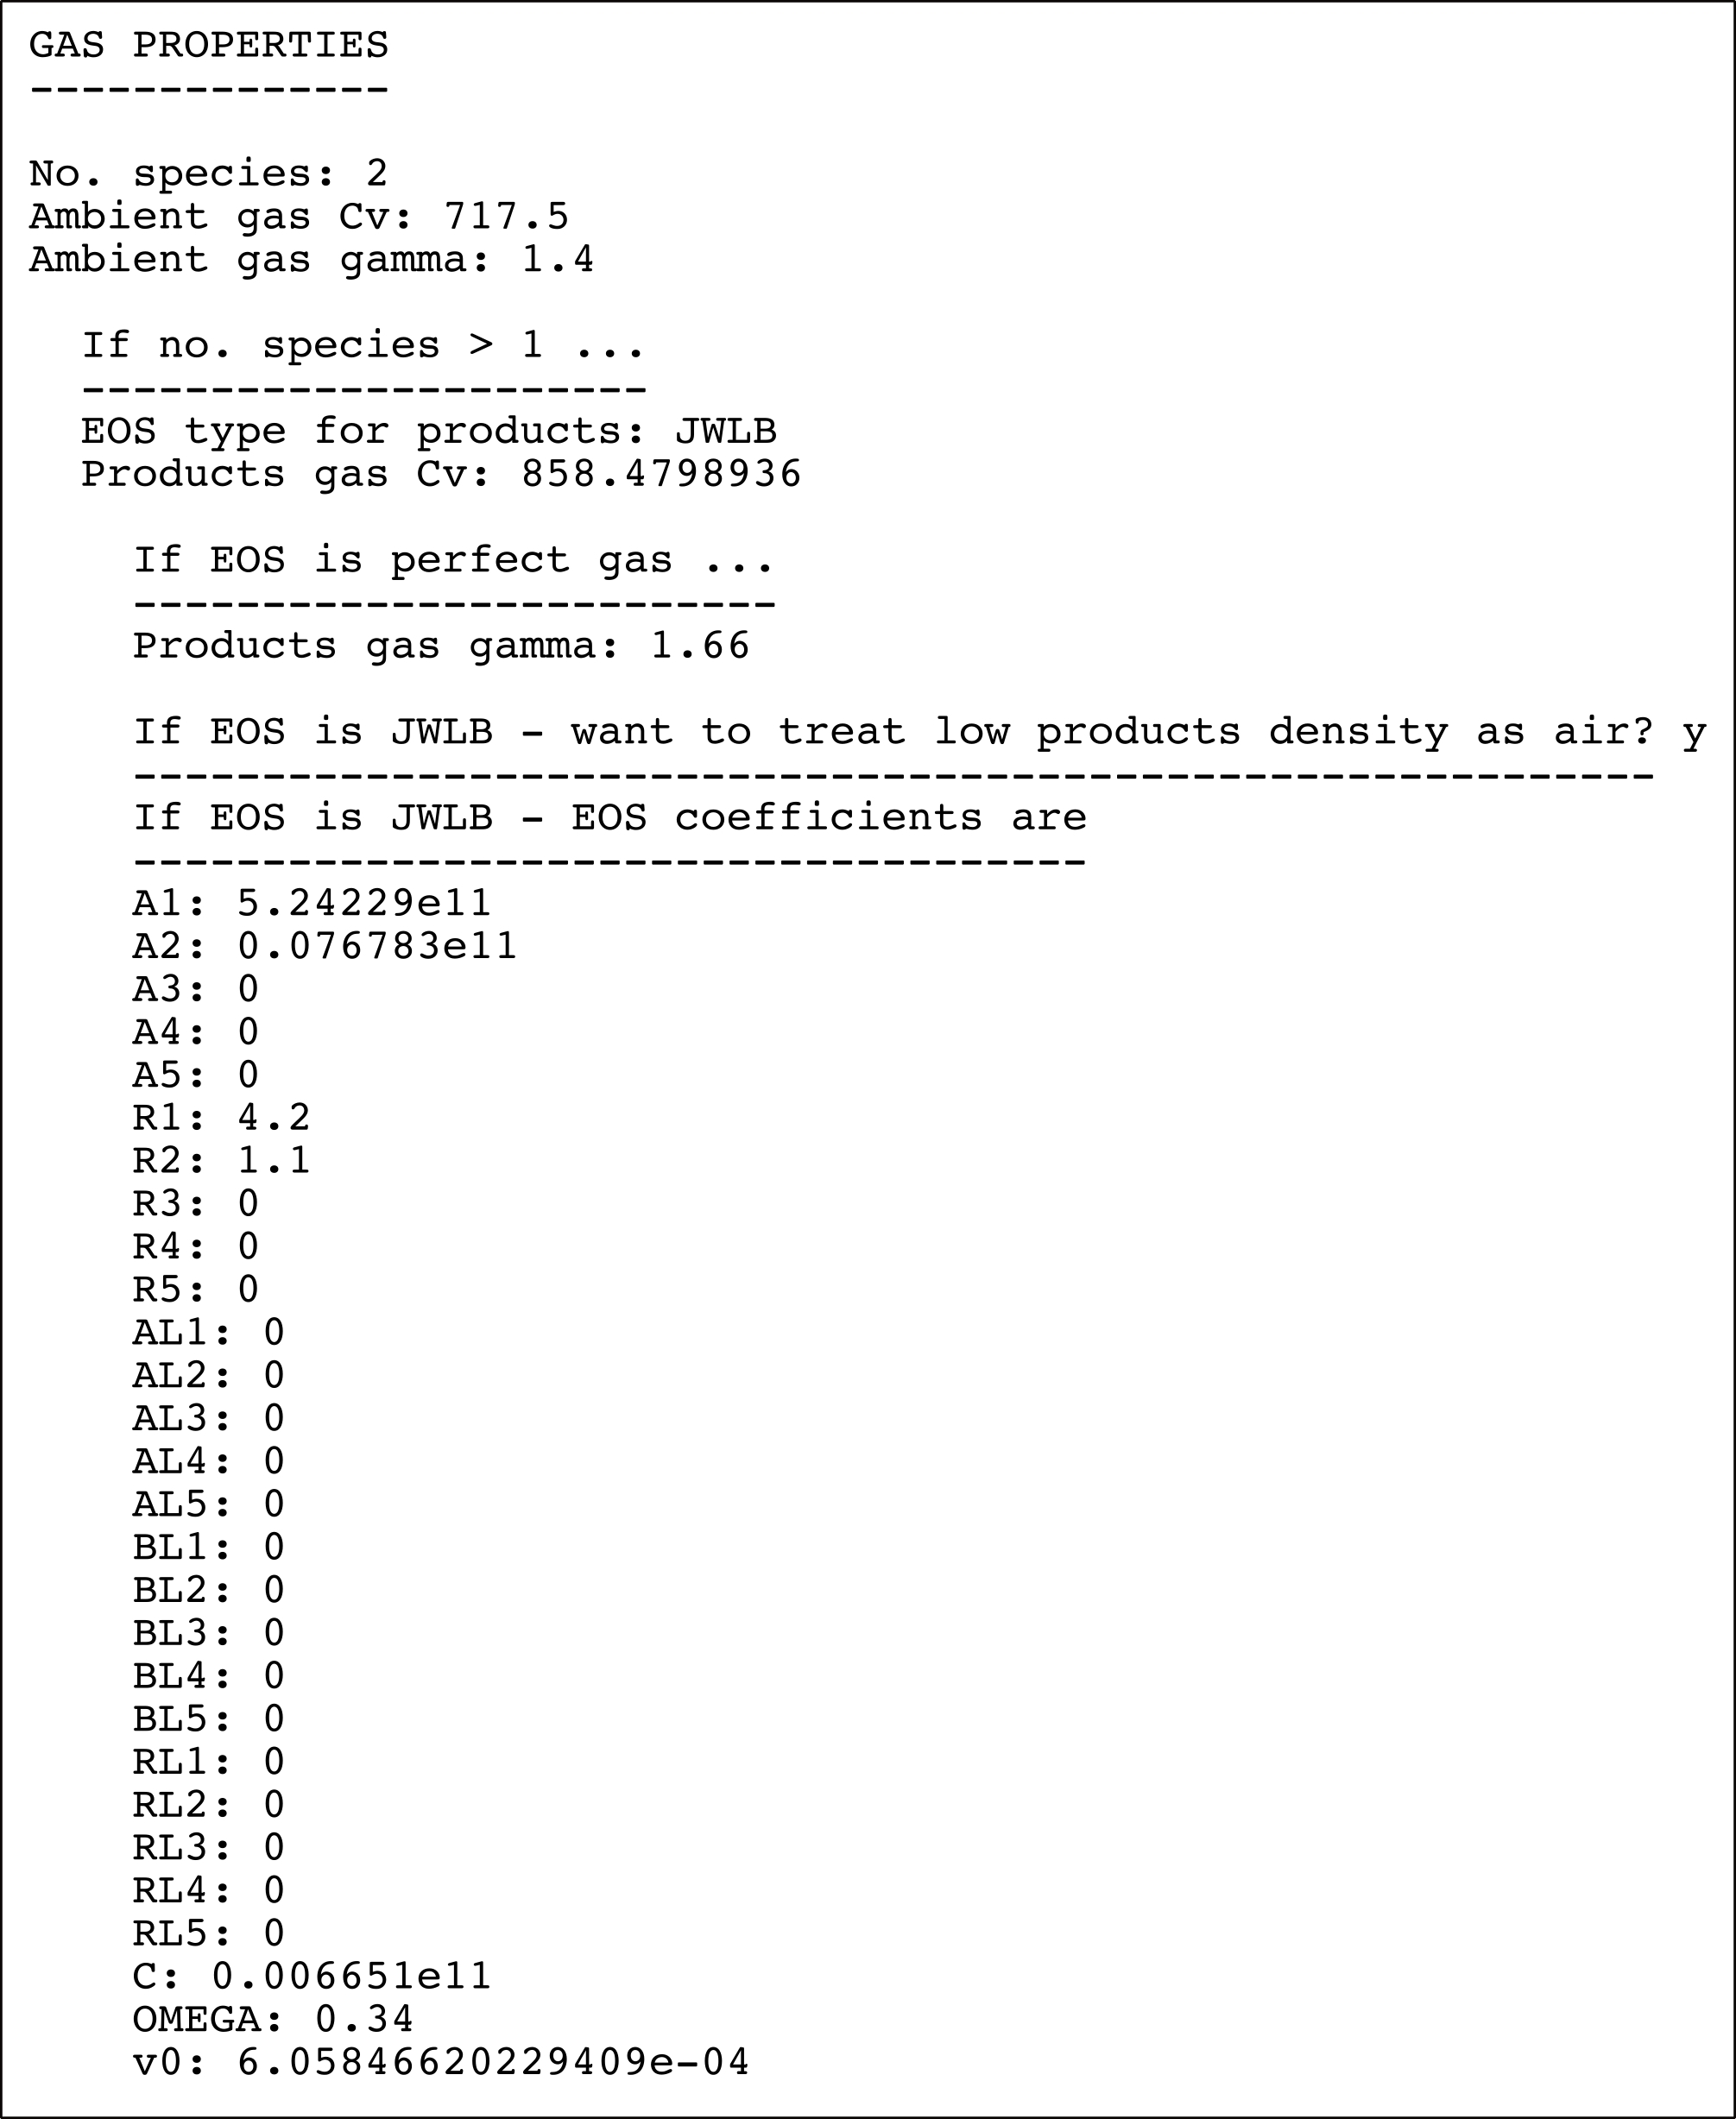
\includegraphics[width=15cm]{pics/ov_gas_template.jpg}
\caption{Gas model file}
\label{fig:ov_gas.par}
\end{figure}
\pagebreak

\section{Domain BC input file}\label{sec:ov_BC}

The domain boundary condition file specifies to OctVCE the boundary conditions that need to be applied to the 6 faces
of the root cell (recall the discussion in $\mathsection$\ref{sec:domain}).  This file must \textbf{follow the format} (with 
\textbf{correct spelling, captials where necessary} etc) of the template in
fig~\ref{fig:ov_BC.par} (a template can also be found in \verb'Octvce3.5.'$\star$\verb'/tests/ov_BC.par').  Note 
that \textbf{any dimensional parameters are assumed to be in SI units}.  

Recall that reflecting (or wall) boundary conditions are \textbf{implemented by the presence of a solid body}, so this file
is really for all other boundary conditions.
The manner of input to this file is somewhat different from other input files described so far, so it might be best to show how this
file is used with the examples in fig~\ref{fig:ov_BC.par} and 
fig~\ref{fig:ov_BC2.par}.  These two examples are probably the only ones that most users need to know.

\subsection{Non-reflecting BCs}\label{sec:non-reflect}

In fig~\ref{fig:ov_BC.par} note that a \verb'Non-reflecting' boundary condition in the ``\verb'BC type:''' field is applied to all 
the faces 
of the root cell (east/west boundaries are perpendicular to the $x$ axis, north/south to the $y$ axis and upper/lower to 
the $z$ axis).  For explosions modelling where boundaries remain `open' to air, the non-reflecting option (based on Thompson's 
formulation \cite{Thompson:bcs}) is probably the most useful.
The non-reflecting BCs nevertheless do cause weak reflections if post-shock flow is subsonic, so a perhaps a better strategy
would just be to extend the domain far enough for the BCs to be a non-issue.

If a solid body obstructs a cell face on a domain boundary, then a solid wall boundary condition is applied there instead of 
whatever is written in this file for that boundary.

\begin{figure}[htp]
\centering
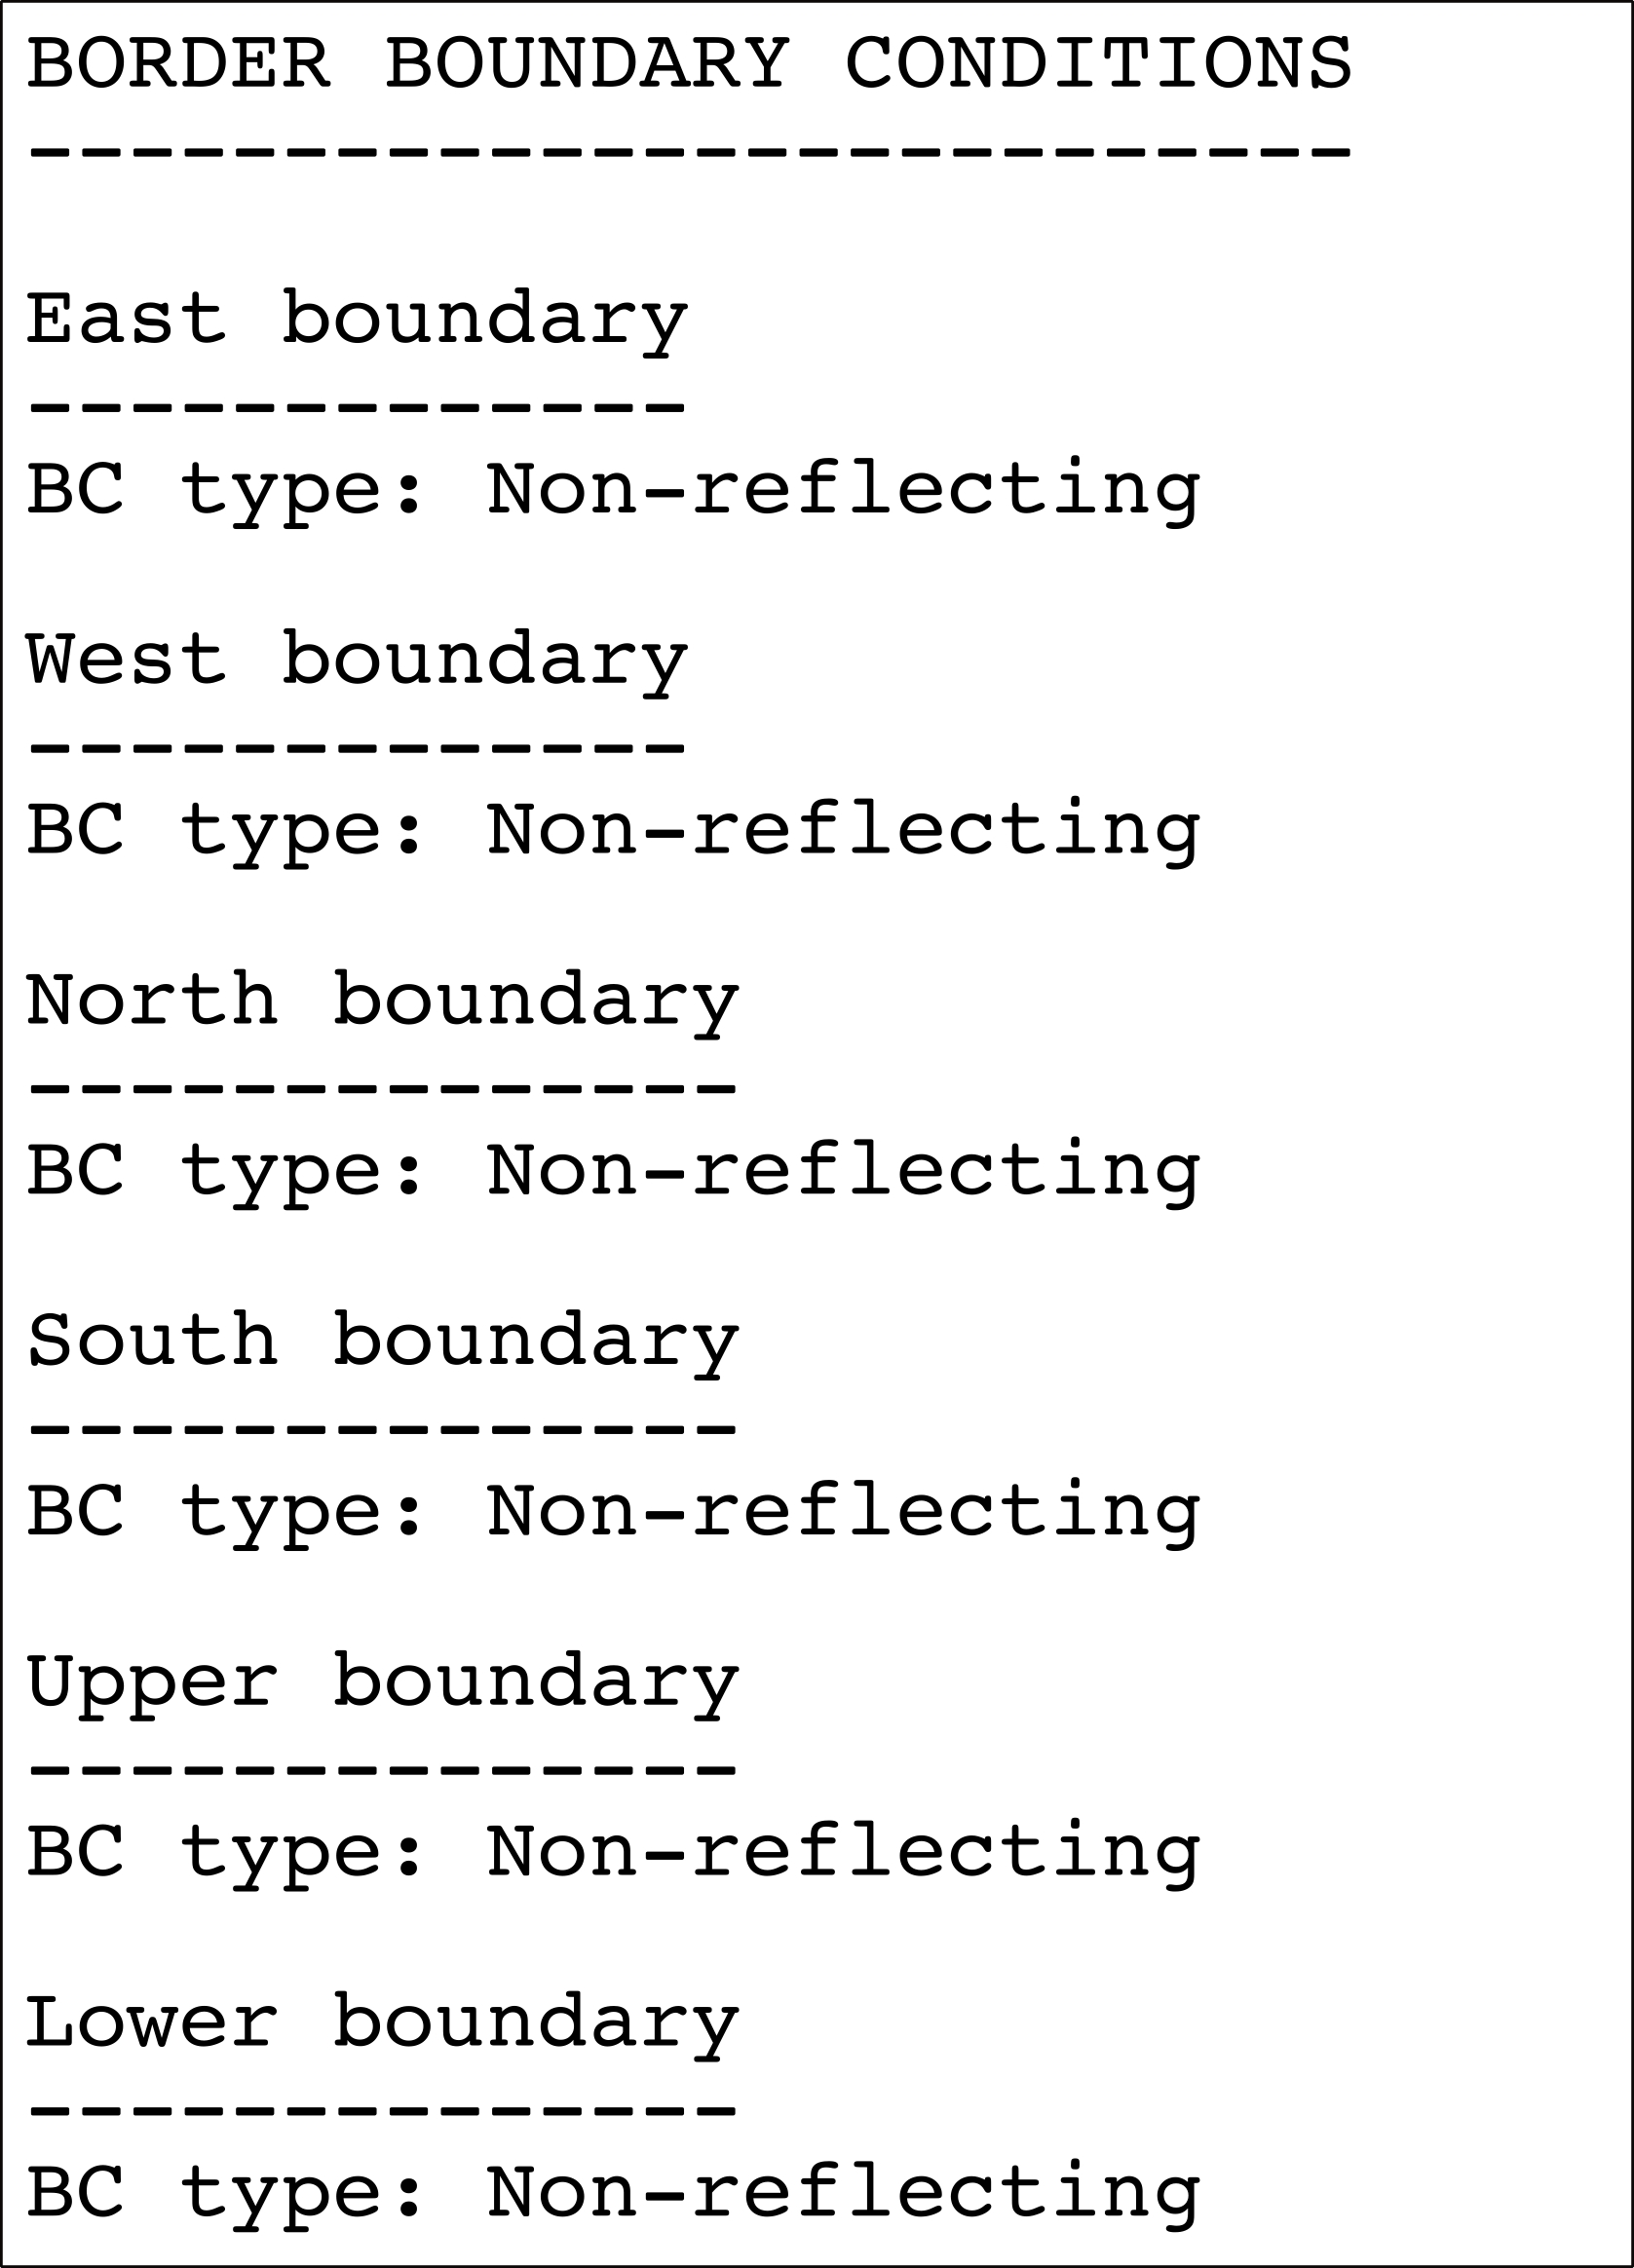
\includegraphics[width=5cm]{pics/ov_BC_template.jpg}
\caption{Example domain boundary condition file}
\label{fig:ov_BC.par}
\end{figure}

\subsection{Inflow and outflow BCs}\label{sec:BC_fixed}

Fig~\ref{fig:ov_BC2.par} specifies a supersonic inflow coming from the west domain boundary with an extrapolated outflow
at the east domain boundary (i.e.\ flow from left to right).  The ``\verb'BC type:''' is now \verb'Specific' as flow variables need to be 
set to a numerical value or to an \verb'Extrapolated' value.  The flow variables that need to be set are the pressure, density 
and velocity.  A similar input can be made on the north, south, upper and lower domain boundaries.   

As noted in $\mathsection$\ref{sec:BC_fixed} if a solid body obstructs a cell face on a domain boundary, then a solid wall boundary 
condition is applied there instead of whatever is written in this file.

\begin{figure}[htp]
\centering
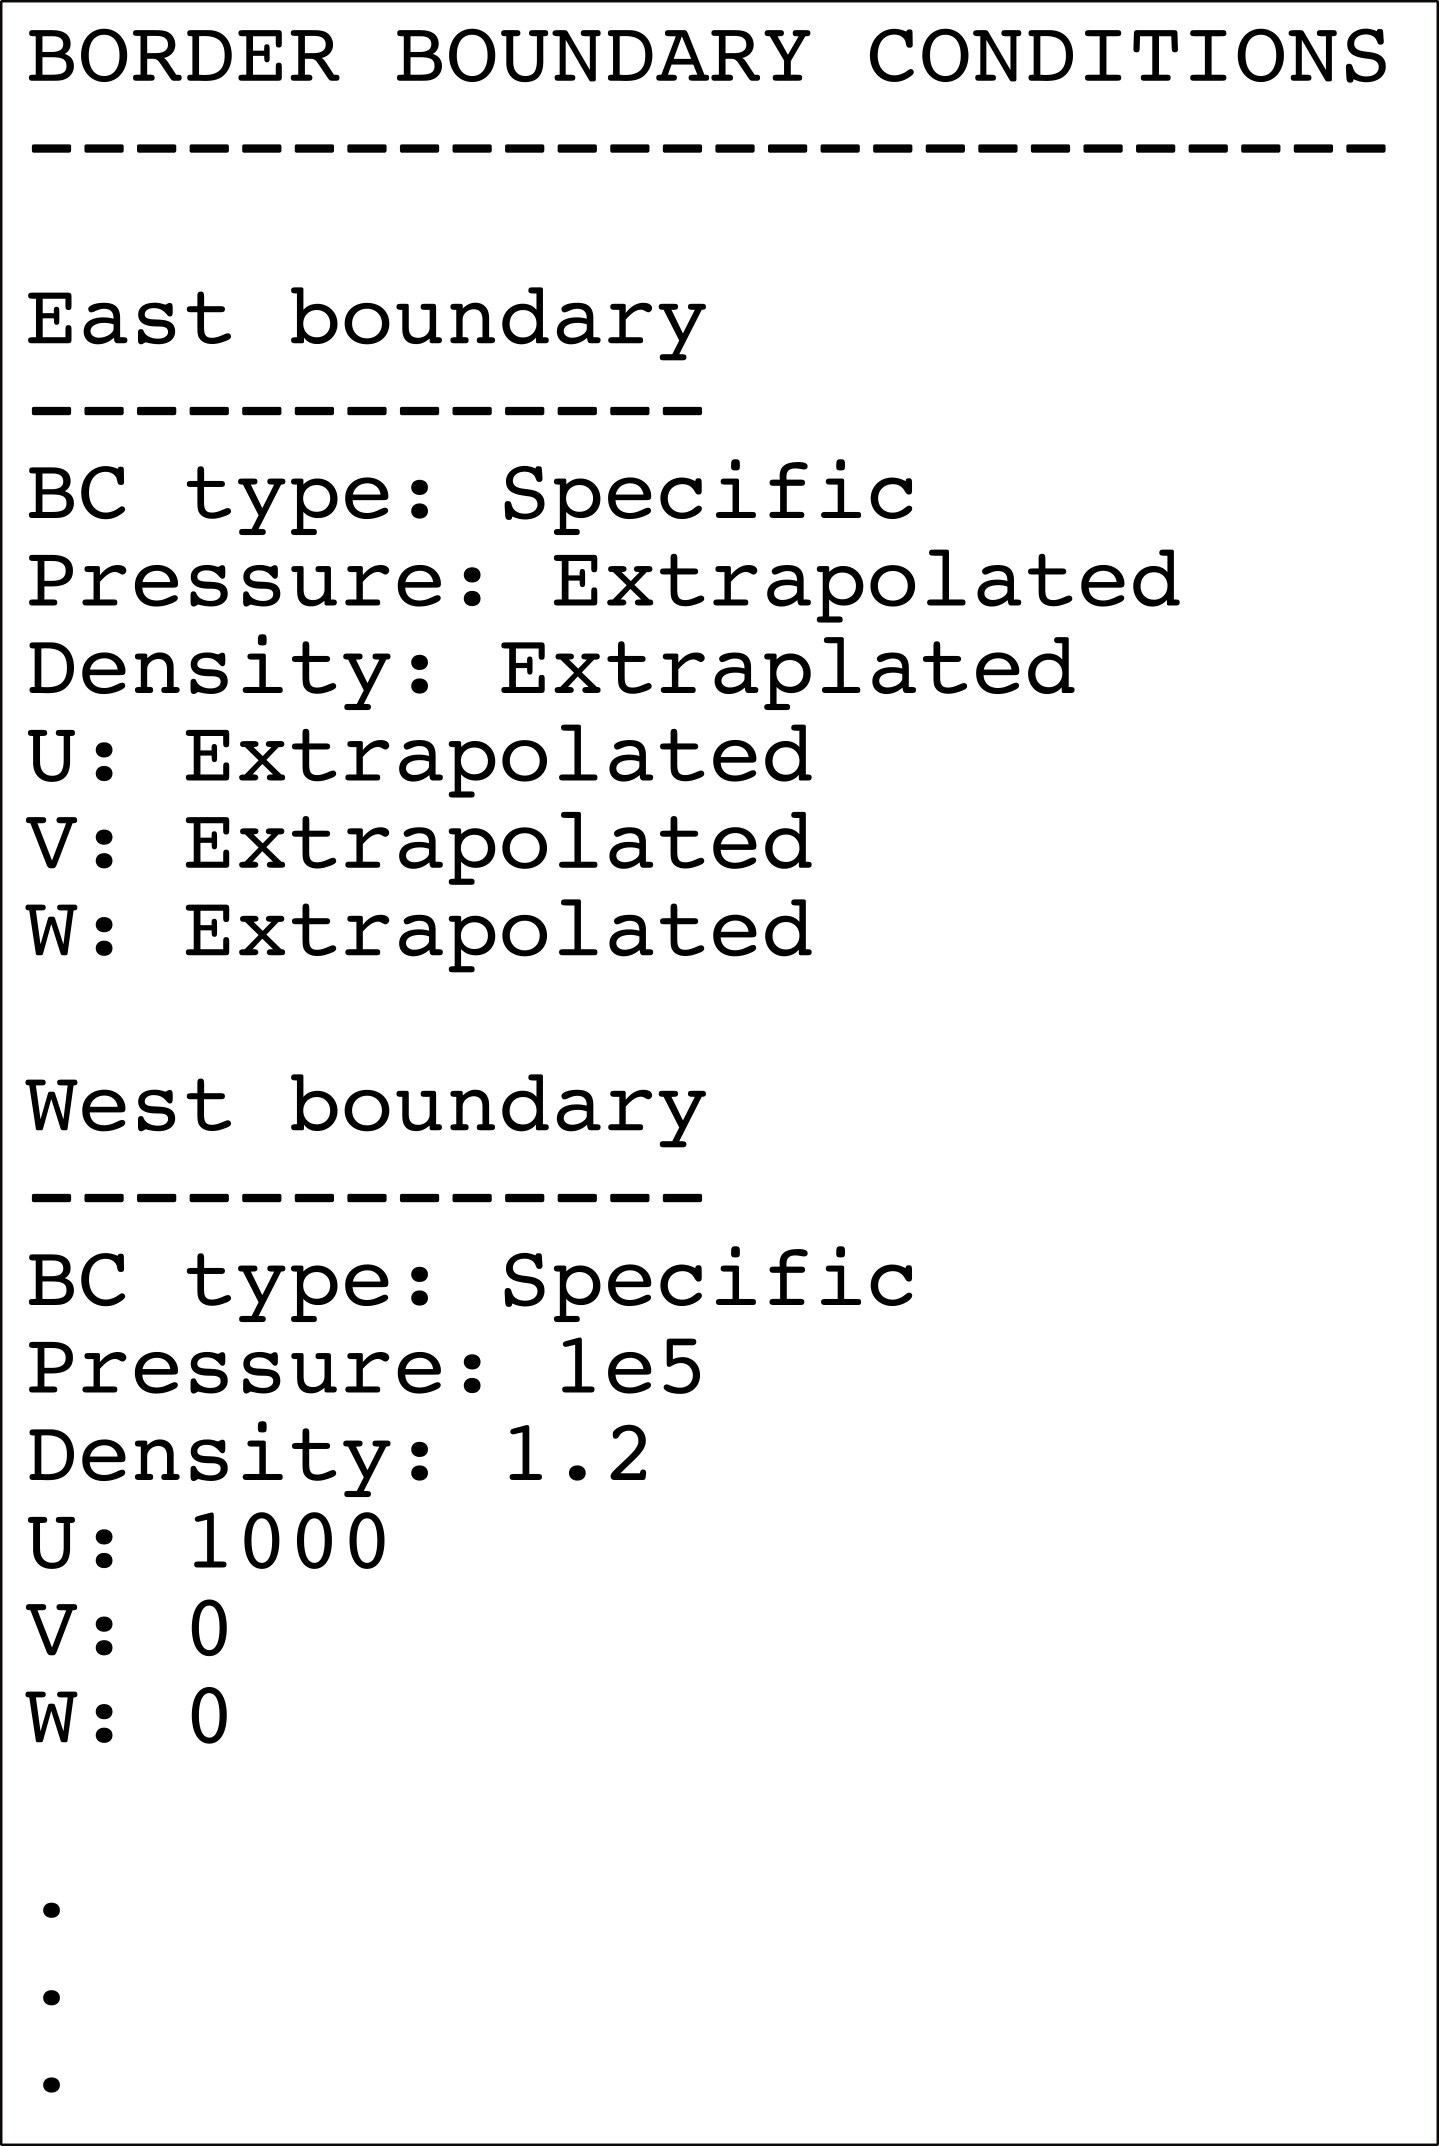
\includegraphics[width=5cm]{pics/ov_BC_template2.jpg}
\caption{Fields for inlet and outlet BCs}
\label{fig:ov_BC2.par}
\end{figure}

\section{`Detonation' data input file}\label{sec:deton}

As mentioned in $\mathsection$\ref{sec:explo} it is possible for `detonation-like' modelling where ignition points are specified
within a solid explosive for detonation waves moving outward from these locations to consume the whole explosive.  The data for the 
ignition points and detonation velocities is specified in the detonation data file.  It must be follow \textbf{exactly the same format}
as the template in fig~\ref{fig:detonations.par} (a template can also be found in \verb'Octvce3.5.'$\star$\verb'/tests/detonations.par').

Note that \textbf{any dimensional parameters are assumed to be in SI units}.  The example in fig~\ref{fig:detonations.par} should not be
difficult to understand.  The user inputs the number of ignition points in the mandatory ``\verb'No. detonation points:''' field.
Then for each ignition point its 3D location and detonation wave radial velocity is written in the
``\verb'Detonation point:''' and ``\verb'Detonation velocity:''' field.

\begin{figure}[htp]
\centering
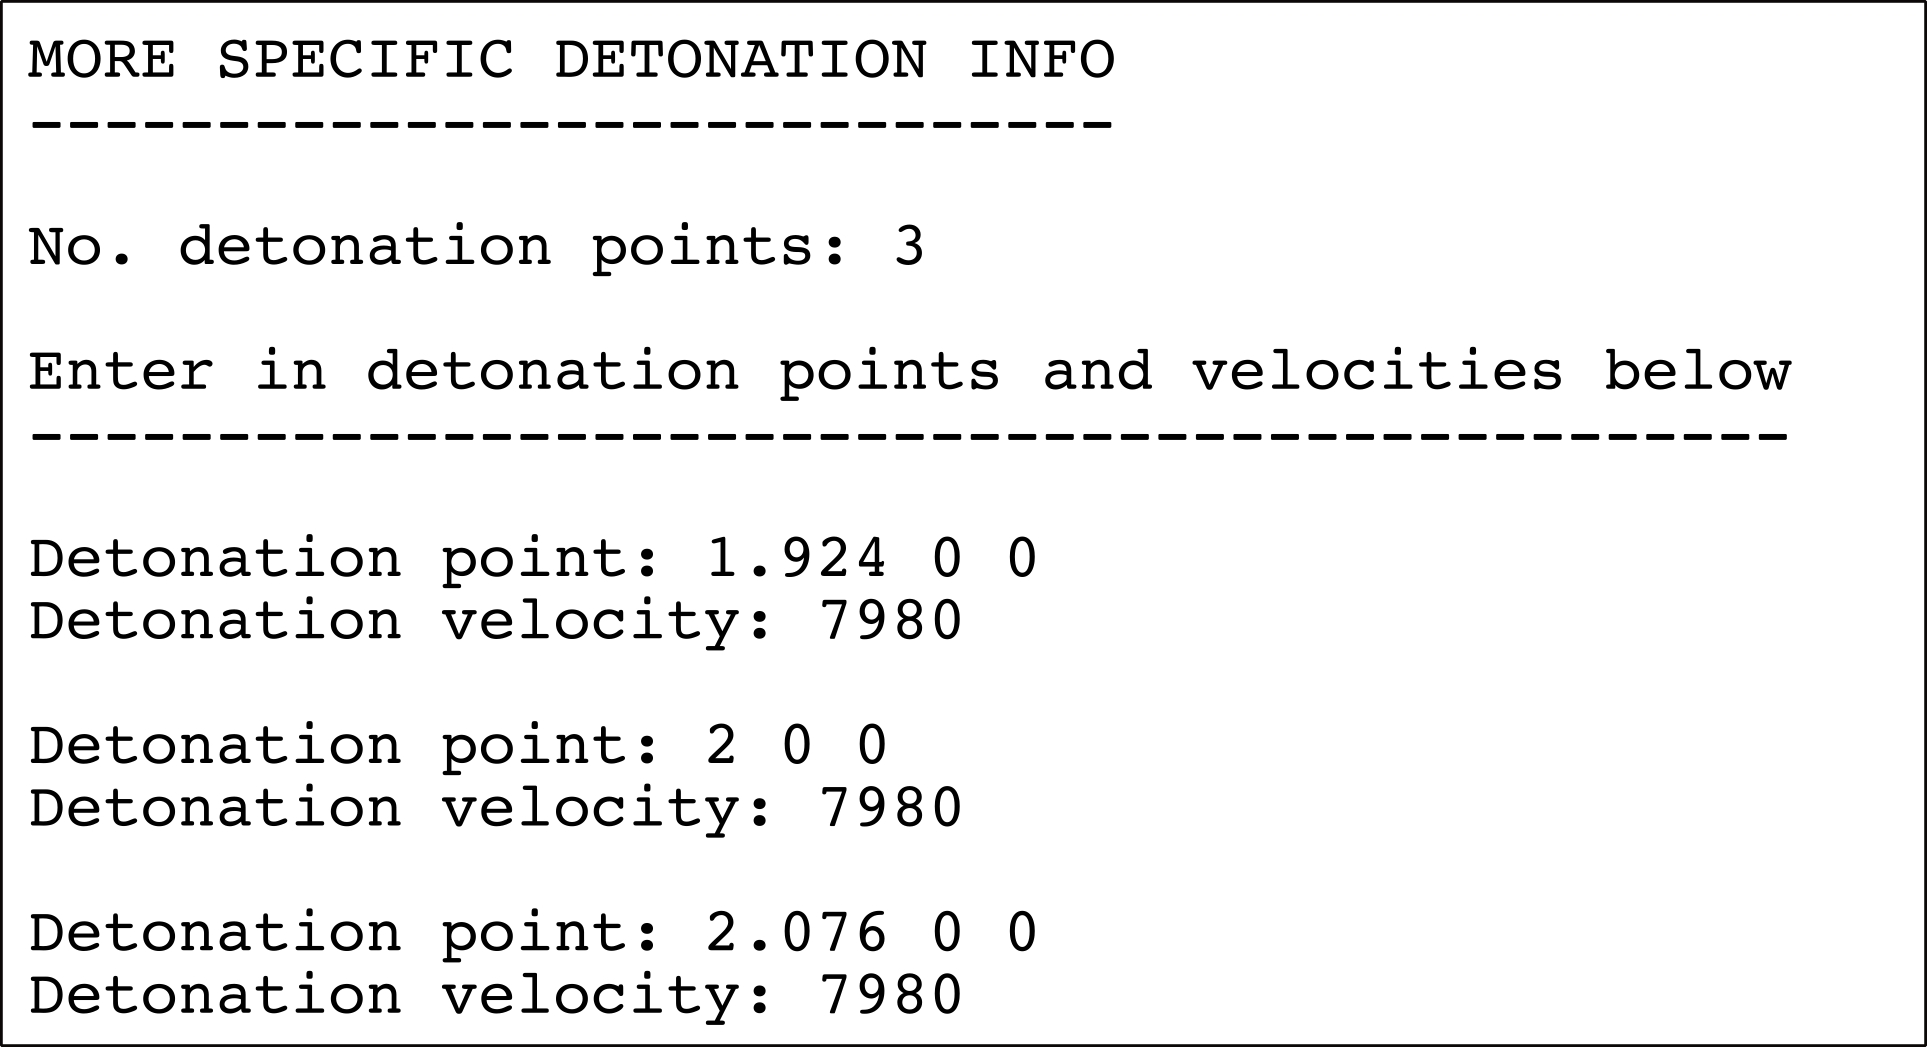
\includegraphics[width=10cm]{pics/deton_template.jpg}
\caption{Example detonation input file}
\label{fig:detonations.par}
\end{figure}

\section{Two-dimensional simulation}\label{sec:2D}

Although OctVCE is a 3D code, 2D planar and axisymmetric simulations in the $xy$ plane can be performed by immersing most of the root cell
in an environment of solid bodies (larger than the root cell) such that only one layer of cells in the $z$ plane is not completely
immersed.  How this is accomplished is discussed in $\mathsection$\ref{sec:2D_thickness} and
$\mathsection$\ref{sec:twoD_subcell}.

\subsection{Making gaps and axes}\label{sec:2D_thickness}

Referring to fig~\ref{fig:yz_plane}, a very thick wall (thicker than the root cell edge) is needed and placed
at $z = t$.  The `lower' $z$ face of the root cell (see $\mathsection$\ref{sec:ov_BC}) \textbf{must be at} $z = 0$.
Later on some command line arguments to OctVCE will be given to let it know a 2D simulation is desired, so the user
need not worry about flow in the $z$ direction.  For axisymmetric calculations, OctVCE assumes the $x$ axis is the symmetric
axis and the $y$ axis is the radial axis.

$t$ is set equal to \emph{half} the length of the highest refined cell, making all 
other leaf cells except those flush with the wall completely immersed, thus giving only one layer of computational cells in 
the $xy$ plane.  $t$ must be set to this value so that all cells including
the smallest ones can have at most two neighbours at a face (consistent with the 2D \emph{quadtree} equivalent of 3D octree adaptation).

\begin{figure}[htp]
\centering
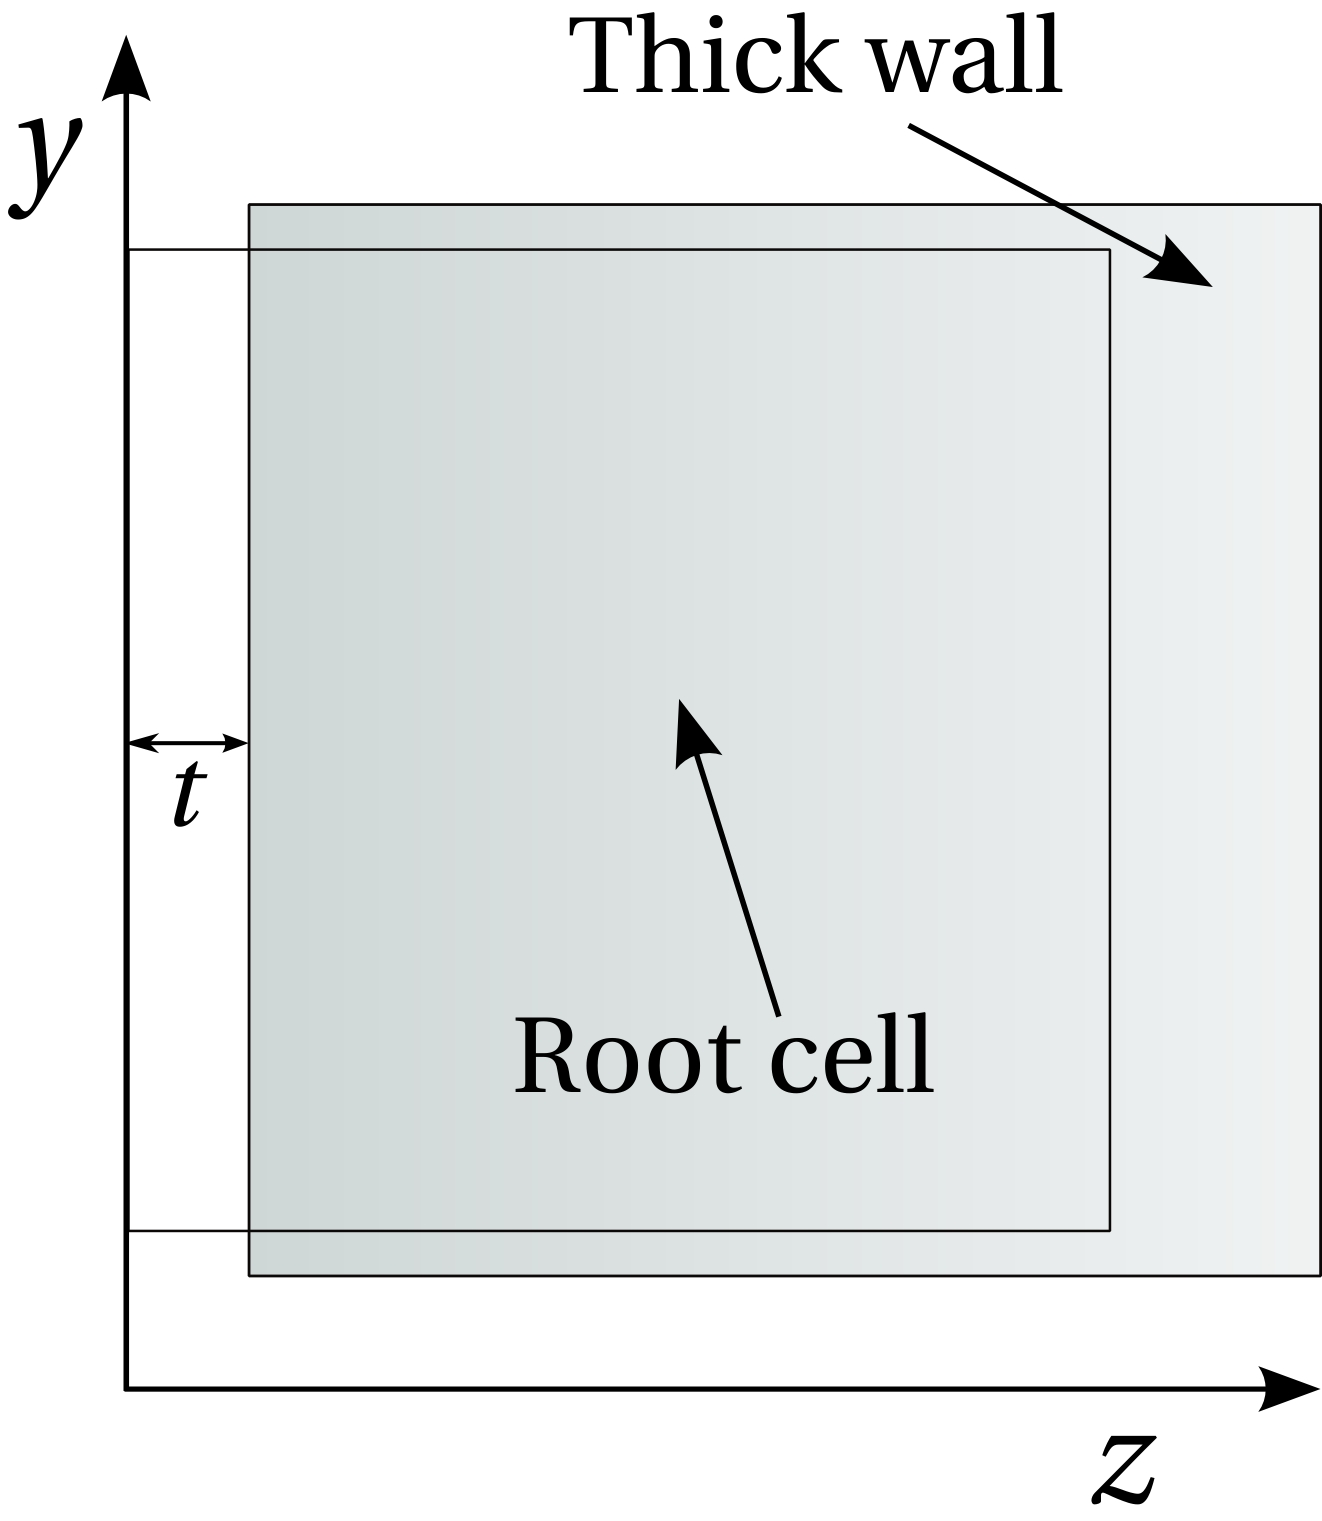
\includegraphics[width=4cm]{pics/twoD_thickness.jpg}
\caption{View from $yz$ plane}
\label{fig:yz_plane}
\end{figure}

\subsection{Caution on axisymmetric computation}\label{sec:axisym_caution}

The inherent nature of VCE means that in axisymmetric geometry there will be some source of conserved quantities produced at
intersected cells.  This is because the approximate surface representation
gives a cell volume (per radian) and area (per radian) and surface normals that are not completely correct.  It might be good to 
run the simulation in quiescent flow with the same geometry to assess the influence of these source terms.  
However, it has been found in practice that these effects are typically quite minor compared to stronger flowfield features, especially 
that resulting from blast.  These effects have also been shown to be small in simple conical supersonic flow \cite{Tang:asm} where
derivation of key quantities of pressure and force are concerned.

\subsection{Appropriate area subcell number}\label{sec:twoD_subcell}

It is also important to ensure that the number of area subcells along a cell edge ($ns_f$ in $\mathsection$\ref{sec:ov_par}) are 
high enough for $t$ to be computed as non-zero (at least one area subcell for the coarsest cell must exist in this
gap).  It is recommended that the $ns_f$ not be lower than 32 for 2D simulations.  If there are 5 levels of refinement (the difference
between maximum and minimum refinement levels), $ns_f$ must be 64, and if 6 levels of refinement, $ns_f$ must be 128 etc.

\chapter{Running a simulation}\label{sec:sim_run}

Remembering that all input files have to be in the same directory as the executable \verb'octvce.exe', the code is then run using the 
arguments --

\verb'./octvce.exe' \verb'-gas' $<$\emph{gas model file}$>$ \verb'-bc' $<$\emph{boundary condition file}$>$ \verb'-ic' $<$\emph{initial condition file}$>$ \verb'-par' $<$\emph{general parameters file}$>$ \verb'-geom' $<$\emph{VTK file of all bodies}$>$ \verb'-ncpus' $<$\emph{no.\ cpus}$>$ [\verb'-deton' $<$\emph{detonations file}$>$] [\verb'-2D'] [\verb'-2D=axisymmetric'] [\verb'-switch-order' $<$\emph{switch time}$>$] [\verb'-output-grid'] [\verb'-output-grid=last'] [\verb'-continue-soln' $<$\emph{mesh file}$>$] [\verb'-count=energy']

The arguments \textbf{in square brackets are optional}; others are mandatory.  Their description will be given below.

\begin{enumerate}
\item \verb'-gas' $<$\emph{gas model file}$>$

Enter in the filename of the gas model input file of $\mathsection$\ref{sec:ov_gas}

\item \verb'-bc' $<$\emph{boundary condition file}$>$

Enter in the filename of the domain BC input file of $\mathsection$\ref{sec:ov_BC}

\item \verb'-ic' $<$\emph{initial condition file}$>$

Enter in the filename of the IC input file of $\mathsection$\ref{sec:ov_IC}

\item \verb'-par' $<$\emph{general parameters file}$>$

Enter in the filename of the general simulation parameters input file of $\mathsection$\ref{sec:ov_par}

\item \verb'-geom' $<$\emph{VTK file of all bodies}$>$

Enter in the filename of the \verb'.pvtp' file describing the environment of all solid objects (see $\mathsection$\ref{sec:geom} and
the example in fig~\ref{fig:XML_eg})

\item \verb'-ncpus' $<$\emph{no.\ cpus}$>$

Enter in the number of CPUs/threads for parallel processing (code must be compiled with an OpenMP compiler).  For no parallel
processing enter in `1' (obviously).

\item \verb'-deton' $<$\emph{detonations file}$>$

\emph{An optional argument}.  If `detonation-like' modelling desired, enter in the filename of the detonation data input file of
$\mathsection$\ref{sec:deton}.

\item \verb'-2D'

\emph{An optional argument}, but use if 2D planar flow is being modelled.  Refer to $\mathsection$\ref{sec:2D} for details on how to
set up the simulation for general 2D simulations.

\item \verb'-2D=axisymmetric'

\emph{An optional argument}, but use if 2D axisymmetric flow is being modelled.  Refer to $\mathsection$\ref{sec:2D} for details on how to
set up the simulation for general 2D simulations.

\item \verb'-switch-order' $<$\emph{switch time}$>$

\emph{An optional argument}.  Sometimes even using a single limiter in a higher-order scheme (as discussed 
in $\mathsection$\ref{sec:ov_par}) is not enough to keep the solution stable (from experience, this might happen if the bomb volume is 
resolved with only a few cells).  As a last resort, this option tells
OctVCE to employ a first-order scheme until \emph{switch time}, after which the second-order scheme is resumed.

Rose \cite[p.g. 61]{Rose:thesis} recommends a scaled switching time of around 1.2 $\times$ 10$^{\text{-3}}$ s/kg$^{\text{1/3}}$
for the explosive mass.

\item \verb'-output-grid'

\emph{An optional argument}.  Will output the whole mesh (tree structure, flow state etc) at the same frequency as solution files
are being output.  Mesh files have a \verb'.ov_out' extension.  The simulation can be continued using these solution files using 
the \verb'-continue-soln' argument (see below).  

\item \verb'-output-grid=last'

\emph{An optional argument}.  Like \verb'-output-grid' of above, but only outputs mesh file at the end of the simulation.

\item \verb'-continue-soln' $<$\emph{mesh file}$>$

\emph{An optional argument}.  Continue the simulation from the mesh file with the \verb'.ov_out' extension generated using
the \verb'-output-grid' option.  The initial condition data from \verb'ov.par' is ignored.

\item \verb'-count=energy'

\emph{An optional argument}.  Used for high explosives modelling, where the total energy and volume of all cells in the initial `bomb' 
volume (see $\mathsection$\ref{sec:explo}) is counted and output.  The program then exits.

This is handy as the cartesian cell `staircasing' representation of the initial bomb volume when the initial grid is generated may 
give total explosion energies that are slightly too high or low.  The information output can be used to ensure a better energy match
by adjusting bomb volume and/or gas condition.  
\end{enumerate}

As the simulation is run some data (like timestep, step number, CFL, no.\ cells refined/coarsened etc) will also be output on the screen.

\section{Memory usage}\label{sec:mem_use}

OctVCE is quite a memory-intensive code, with total memory used per cell during a simulation estimated at around 4 kb.  For this reason 
in large simulations it's necessary to run this code on shared-memory platforms, but this is recommended anyway for obtaining
solutions in a reasonable timeframe.    

\section{Grid convergence and/or error estimation}\label{sec:sim_error}

As with any CFD method where discretization errors exist, it is generally recommended to do a grid convergence study involving
a minimum of two different grids (three preferrably).  In this case, it can typically involve monitoring behaviour at a pressure trace
or group of traces as the grid is refined.  A converging series of traces can be taken as indicative of a converging solution in general.

This allows an estimation of error based on Richardson-extrapolation
(see \cite{Roache:book,Roy:ro}) and possibly a more accurate estimate of the true \emph{numerical} solution, provided 
the grids are fine enough for convergence of the solution to be observed.  How good the true numerical solution corresponds
to the \emph{actual}, or real-world (experimental) solution is a separate validation exercise (several of which are currently
being undertaken by the author).

Generalized Richardson-extrapolation predicts the exact solution $f_{exact}$ to be a function of the finer grid solution $f_1$,
coarser grid solution $f_2$, grid refinement factor $r$, and order of the scheme $p$ as follows in eqn~\ref{eq:Richardson}.

\begin{equation}\label{eq:Richardson}
  f_{exact} = f_1 + \frac{f_1 - f_2}{r^p - 1}
\end{equation}

It can be also used to predict quantites derived from the solution e.g.\ surface force.  The second term in eqn~\ref{eq:Richardson}
can be thought of as the `error' as it represents an additive correction to $f_1$, and is a reasonable approximation to the
true numerical error when it is much smaller than $f_1$.  

As OctVCE only allows integer halvings of cell sizes, $r = 2$ nominally.  This inherently assumes that the solution on an
adapted mesh is just as good as the solution on a uniform mesh with the same minimum cell size, which is not always true in general.
$p$ can be between $1$ and $2$ depending on what quantity is being measured e.g.\ peak overpressure would be best
with $p = 1$ as it's a shock-dependent quantity and the present scheme is first order at shocks.  In smoother flow regions,
$p$ can be nominally $2$ as OctVCE is a nominally second-order method (though a value between $1$ and $2$ might be more reasonable due to
the presence of limiters and other numerical effects that can hamper the solution order).   

\chapter{Post-processing}\label{sec:post_proc}

\section{Solution file format}\label{sec:soln_file}

Solution files are also in the VTK XML version 4.2+ ASCII file format (see $\mathsection$\ref{sec:geom}) but will have a name of 
\emph{basename}\verb'.'$\star$\verb'.vtu' and/or \emph{basename}\verb'.'$\star$\verb'.pvtu', where \emph{basename} is
the base solution file name (see $\mathsection$\ref{sec:ov_par}) and $\star$ the timestep at which the solution file was output.  

If the code was run in serial the solution files will only have the \verb'.vtu' extension.  But if 
the code was run in parallel
on $n$ CPUs, there will be $n$ \verb'.vtu' files corresponding to the mesh portions allocated to each CPU.  All these files
are listed in the \verb'.pvtu' file to comprise the entire mesh domain (recall the discussion on parallel VTK files 
in $\mathsection$\ref{sec:geom}).  For later visualization it is thus the \verb'.pvtu' file that needs to be opened.

\section{Visualizing solution files}\label{sec:viz}

The solution files can only be opened with a VTK file visualizer (obviously).  Two currently existing VTK visualizers are
the Mayavi\footnote{http://mayavi.sourceforge.net/} and Paraview\footnote{www.paraview.org} applications.  Paraview seems to be more
efficient for visualizing very large solution files.  Both these applications can display the solution on a 2D plane (which is usually
desired).

\subsection{A note on displaying 2D solutions}\label{sec:2Dviz}

Recall the disussion on simulation set-up for 2D simulations in $\mathsection$\ref{sec:2D}, where the rest of the root cell
is `trimmed' so that only one layer of cells on the $z$ plane are actually in the flow solution.  However these cells are
nonetheless still three-dimensional.

To fully display the 2D simulation, a planar cut (in the visualizer) must be made such that the plane passes through \emph{all}
cells in this layer (even the finest ones).  If this does not happen there will appear `gaps' in the solution.
So if the lower boundary of the root is at $z = 0$, a $z$-plane cut
at some very small number (say $10^{-10}$) should pass through all cells and the whole 2D solution on this plane will be displayed.

\section{Pressure trace format}\label{sec:p_trace_file}

When pressure traces/histories at a gauge location are recorded (see $\mathsection$\ref{sec:ov_par}), the pressure trace file
for each location records 2 quantities -- (i) the time and (ii) the \emph{overpressure} (pressure minus ambient pressure).  It has 
the name of \emph{basename}$\star$\verb'.dat', where \emph{basename} is the base history filename and $\star$ the trace 
number (starting at 0), corresponding to the order in which the gauge
locations were entered in general simulation parameteers input file ($\mathsection$\ref{sec:ov_par}).  

The file can be read and plotted by gnuplot\footnote{http://www.gnuplot.info/}.  
The trace can yield impulse data by for example placing the columns in an array and writing an  
Octave\footnote{http://www.gnu.org/software/octave/} script to integrate the pressure trace $\int Pdt$.  However as trace files
can get quite large, it might be better to write an integration routine in a more efficient language like C or FORTRAN.

%\begin{figure}[htp]
%\centering
%\begin{verbatim}
%# Pressure trace at location x y z
%trace = [t1 p1 p1/p_amb
%t2 p2 p2/p_amb
%.
%.
%.
%];
%\end{verbatim}
%\caption{Pressure trace file format}
%\label{fig:ptrace}
%\end{figure}

\newpage

\appendix
\chapter{A useful 1D code}\label{sec:useful_tool}

This section describes a useful stand-alone 1D code that has been developed alongside OctVCE for general blast
modelling work.  The 1D code \verb'blast_1D' is much like OctVCE but much simpler to use and faster to run.  It can be run assuming 
planar, cylindrical or spherical symmetry.  The 1D assumption means that the bomb can be thought of as a \emph{driver gas} (as in a 
shock tube) which is 
initialized to the proper explosive conditions.  Like OctVCE, it is a nominally 2nd-order code that uses much of the same
underlying numerical methodology.   

The code is located in the \verb'blast_1D' directory.  The code is compiled in the same way as OctVCE 
is (see $\mathsection$\ref{sec:code_compile}) using the \emph{makefile} in the \verb'blast_1D/unix/' directory.
The default directory where the executable \verb'b1d.exe' is placed is in \verb'blast_1D/tests/'.

Like OctVCE, several input files are required for \verb'blast_1D' to run.  Templates for these input files can be found in
\verb'blast_1D/tests/'.  They are \verb'b1d_gas.par' (gas model input file), \verb'b1d_ic.par' (IC input file) and \verb'b1d.par'
(general simulation parameters input file).  Like OctVCE's input files, the formats of these files cannot be altered (only the
parameters) and they must be in the same directory that the executable \verb'b1d.exe' is in.

The gas model input file is identical to OctVCE's gas model input file (see $\mathsection$\ref{sec:ov_gas}).
The initial condition input file is very simple and simply requires one to specify the initial ambient and driver gas conditions 
(fig~\ref{fig:b1d_ic.par}), like with OctVCE's input file.

\begin{figure}[htp]
\centering
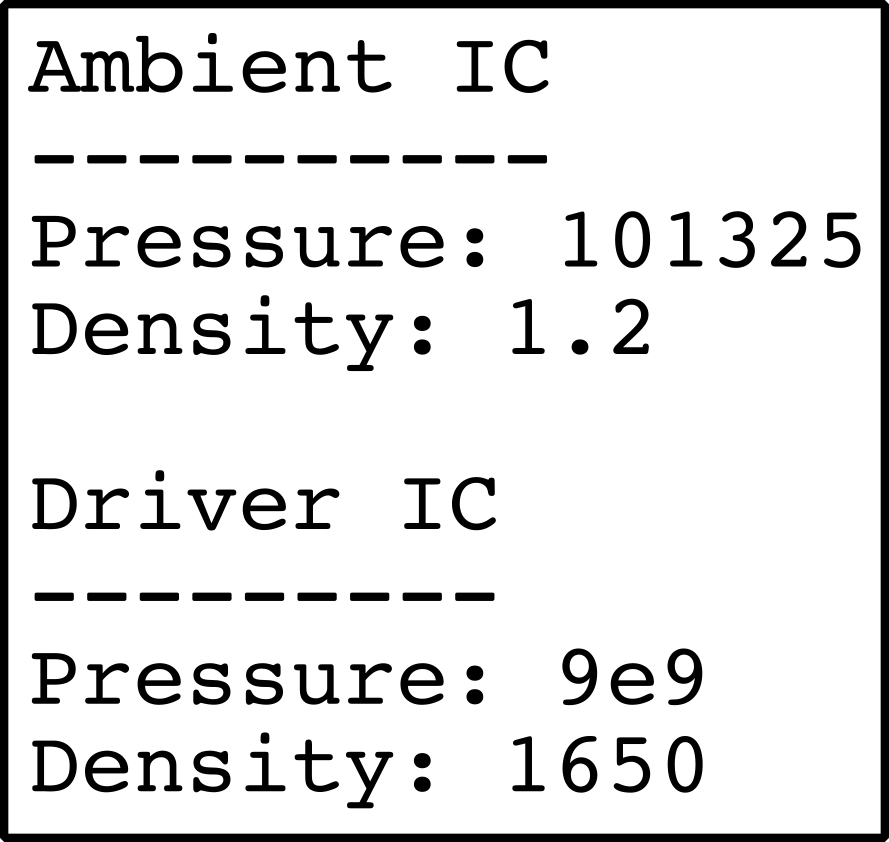
\includegraphics[width=3cm]{pics/b1d_ic_template.jpg}
\caption{IC input file for 1D code}
\label{fig:b1d_ic.par}
\end{figure}

The general simulation parameters input file format can be seen in fig~\ref{fig:b1d.par}.  A description of each input line is
given below.

\newpage

\begin{figure}[htp]
\centering
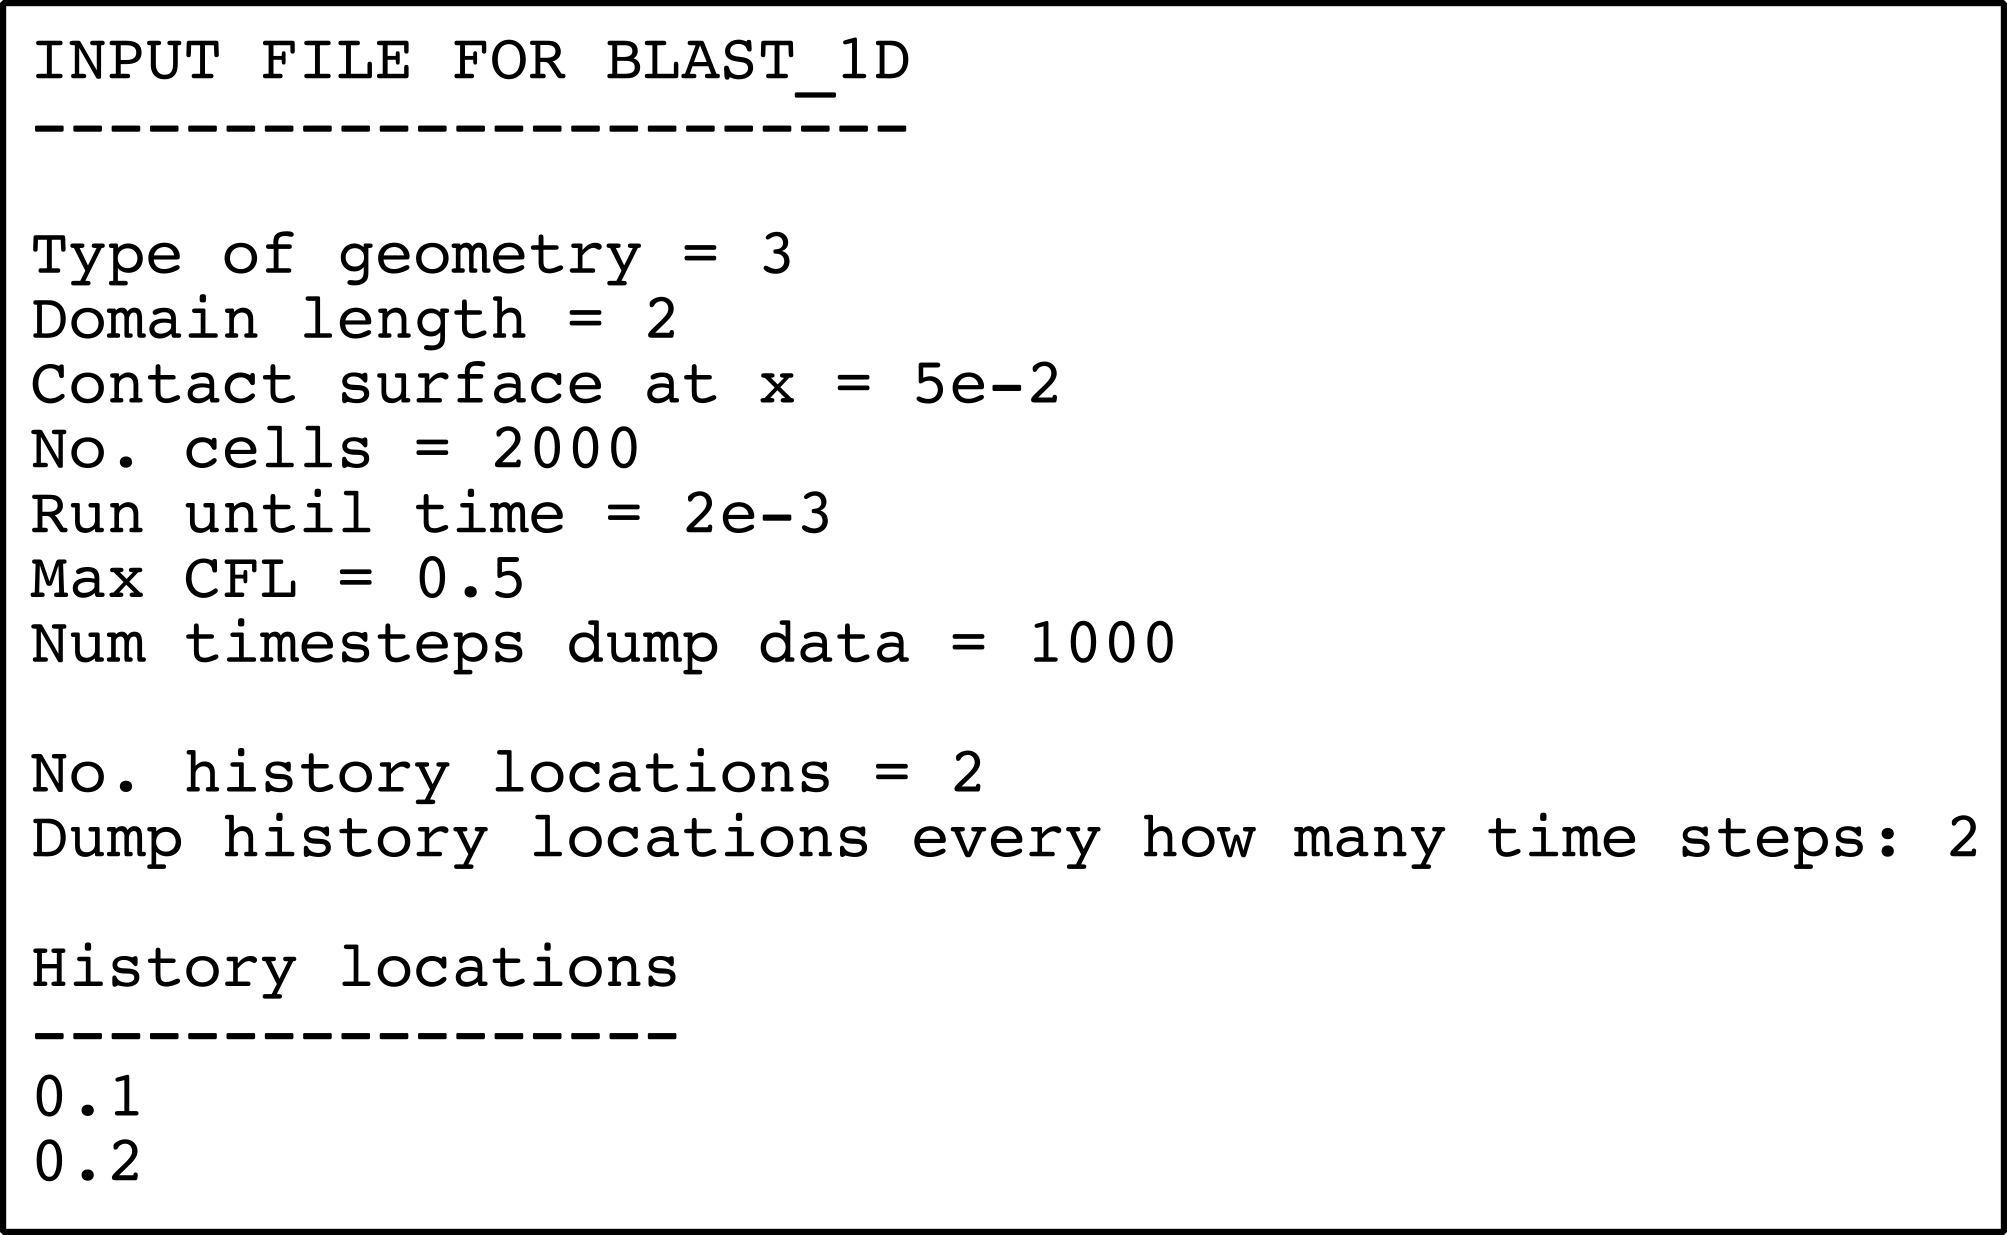
\includegraphics[width=11cm]{pics/b1d_par_template.jpg}
\caption{General parameters file for 1D code}
\label{fig:b1d.par}
\end{figure}

\begin{enumerate}

\item \verb'Type of geometry = ' -- enter \verb'1' for planar geometry, \verb'2' for cylindrical, and \verb'3' for spherical geometry.

\item \verb'Domain length = ' -- enter in length of domain.  Bomb is located at the left end; the right end is set to nonreflecting
  outlet.

\item \verb'Contact surface at x = ' -- enter in location of interface between driver and ambient gas.  For a 1D spherical 
  bomb calculation, this is just the radius of the charge.

\item \verb'No. cells = ' -- enter in the number of cells.  

  Note that it's important to specify a domain length and number of cells so that there are an integer number of cells within
  the charge, thus matching bomb energy exactly.

\item \verb'Run until time = ' -- enter in time where simulation finishes

\item \verb'Max CFL = ' -- enter in maximum CFL; usually 0.5 is a good number.

\item \verb'Write data frequency = ' -- output frequency (with respect to solution time) of solution.

  The solution files will have a \verb's.'$\star$\verb'.dat' name where $\star$ is the timestep at which the solution was output.
  The columns of this \verb'.dat' file consist of cell location, density, pressure, products mass fraction and flow velocity,
  and it can be easily plotted by gnuplot\footnote{http://www.gnuplot.info/}.

\item \verb'No. history locations = ' -- the number of pressure gauges desired

\item \verb'Dump history locations every how many time steps = ' -- how often should the pressure at a point be recorded.  Typically recording every 2 to 5 timesteps is enough.

At each line below the \verb'History locations' line, enter in the gauge location (along the x-axis, as this is a 1D case) where
the pressure trace is recorded.  Each trace file has a \verb'hist_'$\star$\verb'.dat' name where $\star$ is the
trace number (starting at 0) corresponding to the order in which the gauge locations were entered.

\end{enumerate}

\chapter{Example simulations}\label{sec:sim_eg}

This section will cover some example simulations which are included with the source code in
\verb'Octvce3.5.'$\star$\verb'/tests/' (all geometry and input files are provided).  Additional explanations are provided
where appropriate.  It is hoped that these examples will help the user get started easily and relatively quickly
with the OctVCE code (though reading the material in $\mathsection$\ref{sec:sim_setup} to $\mathsection$\ref{sec:sim_run} is also
recommended, of course).  Some results will also be provided.

\section{Supersonic conical flow}\label{sec:cone_eg}

Here supersonic flow over a cone with a $20^{\circ}$ half-angle is simulated (post-shock $M_{\infty} = 1.5$, whilst shock $M = 3.66$).
This is a 2D axisymmetric simulation.  The geometry and input files are in \verb'Octvce3.5.'$\star$\verb'/tests/cone_eg/'.

\subsection{Cone geometry}\label{sec:cone_geom}

As this is an axisymmetric simulation, the geometry must be constructed in the manner described in $\mathsection$\ref{sec:2D}.
The $x$ axis is the axis of symmetry and $y$ the radial co-ordinate.

The geometry files for individual bodies are \verb'ceiling.vtp' (to prevent flow out the top $y$ 
boundary), \verb'cone_20.vtp' (the actual cone geometry) and \verb'floor.vtp' 
(to prevent flow out the bottom $y$ boundary).  Note how the ceiling and floor very slightly overlap the domain (recall
the discussion in $\mathsection$\ref{sec:grid_flush}). 

Finally the required `thick wall' (to ensure only 1 layer of cells in the $z$-plane -- see $\mathsection$\ref{sec:2D_thickness}) 
is file \verb'right_wall.vtp'.  All these bodies are listed in the parallel VTK
file \verb'bodies.pvtp' describing the environment.  The whole geometry is displayed in fig~\ref{fig:cone_geomfig}.

\begin{figure}[htp]
\centering
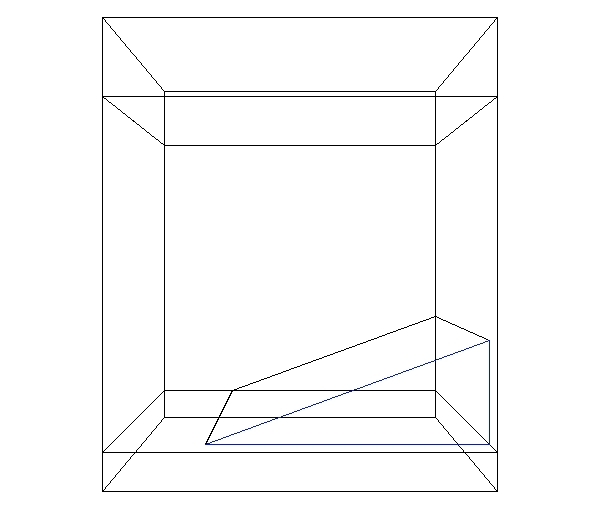
\includegraphics[width=5cm]{pics/cone_eg/geom.jpg}
\caption{Geometry for cone simulation}
\label{fig:cone_geomfig}
\end{figure}

\subsection{Input files for cone simulation}\label{sec:cone_par}

All input files are located in \verb'Octvce3.5.'$\star$\verb'/tests/cone_eg/*.par'.  

\subsubsection{General simulation parameters file}

This file has been called \verb'ov.par'.

\subsubsection{IC input file}

This file has been called \verb'ov_IC.par'.

Note the IC input file has 2 initial conditions for the ambient and `explosive products' gases.
However in this case it is better to think of the `explosive products' gas as simply the gas at \emph{post-shock} conditions.  Rather
than staring the simulation with flow coming in from the left boundary, some computation time can be saved if the initial conditions
are setup so that the shock has already entered the domain but not passed the cone.  

This approach is also advantageous if mesh refinement at the shock is desired (though this isn't done here), as if
the simulation starts by having the shock enter the domain, it isn't possible under the current input method for the mesh to be 
refined to the maximum level around the shock if no post-shock initial condition already exists \emph{in the domain}.  
As discussed in $\mathsection$\ref{sec:ov_IC} it is necessary to have a file describing the geometry of the bomb volume (or in this
case, the post-shock flow), and this is given in \verb'ic.vtp'.

\subsubsection{Gas model input file}

This file has been called \verb'ov_gas.par'.  Note only 1 (ideal-gas) species is necessary (though there are 2 regions where the initial 
pressures, densities and velocities are different -- see above).

\subsubsection{Domain BC input file}

This file has been called \verb'ov_BC.par'.
As this simulation has supersonic inflow coming from the west (or left) with extrapolated outflow at the east (or right) boundary,
the domain BC input file follows nearly exactly format as discussed in $\mathsection$\ref{sec:BC_fixed} (with only the values different).
It is necessary to enter in `boundary conditions' for the other root cell faces, even though solid wall boundary conditions
are set for them.  

\subsection{Running the cone simulation}\label{sec:cone_run}

Now that all input files have been appropriately created, the code is run with the command line arguments as shown below (recall
the discussion in $\mathsection$\ref{sec:sim_run}).  As this code was run on a 2 CPU SMP, 2 CPUs have been used.

\begin{figure}[htp]
\centering
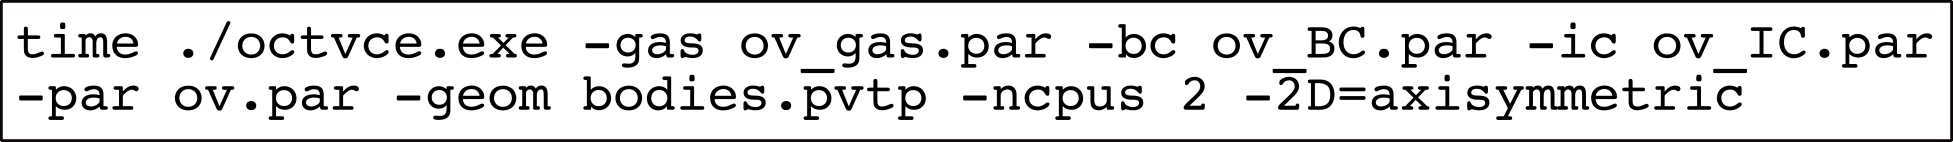
\includegraphics[width=14cm]{pics/cmd_exe_cone.jpg}
\caption{Running the cone simulation}
\label{fig:cone_run}
\end{figure}

Some screen output from the first 2 timesteps is shown below.  Note that at present adaptation in parallel for 2D simulations
isn't done as total numbers of cells aren't very large, giving relatively small benefit from the extra work (recall the discussion
in $\mathsection$\ref{sec:ov_par}).  The number of computational cells is 52555.

\begin{figure}[htp]
\centering
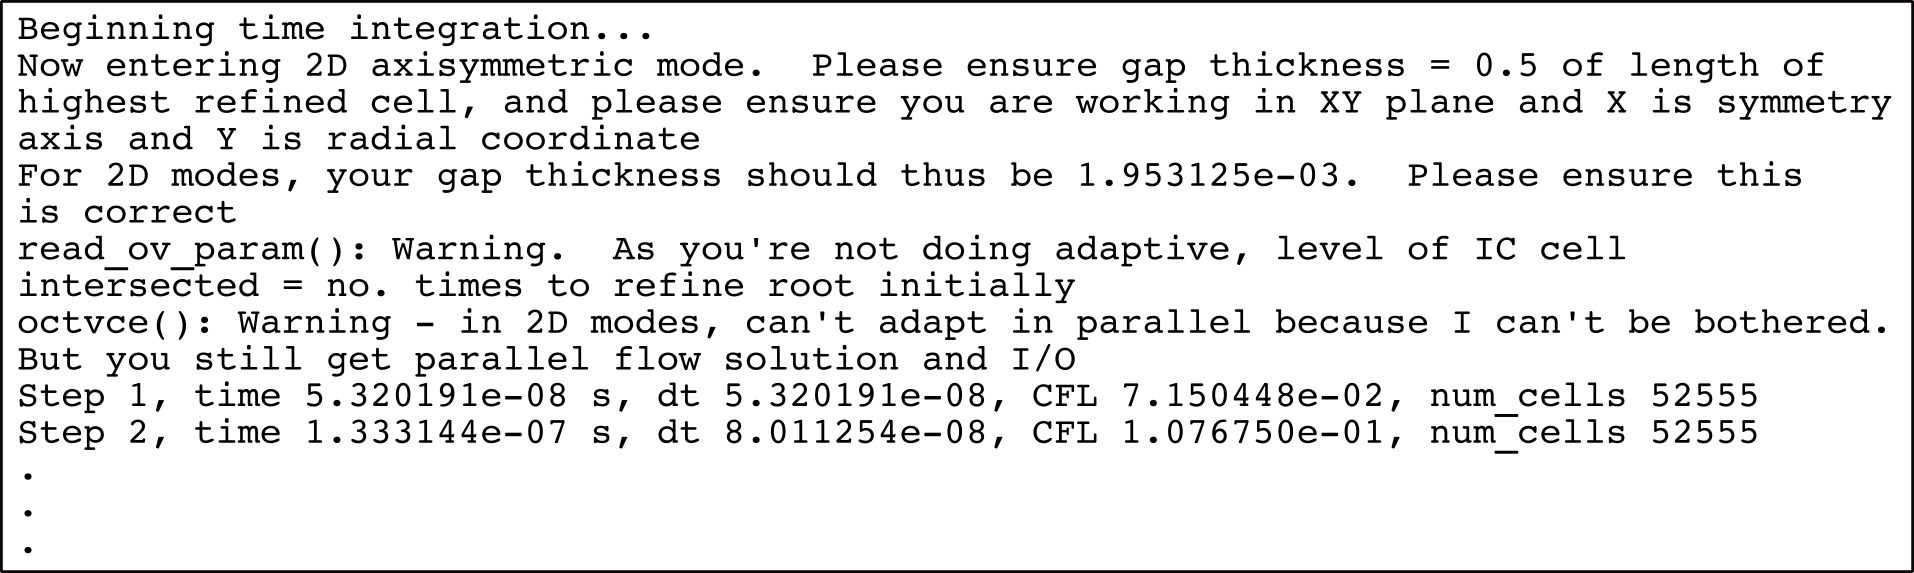
\includegraphics[width=16cm]{pics/cone_output.jpg}
\caption{Some screen output from cone simulation}
\label{fig:cone_output}
\end{figure}

\subsection{Some results for cone simulation}\label{sec:cone_results}

The initial solution is shown in fig~\ref{fig:cone20_r_0} where the 2 different initial conditions (for ambient and post-shock
flow conditions) can be easily seen.  Fig~\ref{fig:cone20_r_us1} shows the density contours at 0.5 ms before the shock has exited
the right boundary.  It can be seen that the reflected shock, Mach stem and contact discontinuity are captured quite well.

In the steady state limit (fig~\ref{fig:cone20_r_s1}) one can see some `noise' existing at the surface.  This arises from the inherent 
nature of VCE
in approximating surfaces (a more detailed disucssion is given in \cite{Tang:asm}).  However the solution should be sufficient for
practical engineering purposes, with the shock angle agreeing very well with the theoretical result (the black line).

\begin{figure}[htp]
  	\centering
	\subfigure[Initial solution]{
	  \label{fig:cone20_r_0}
	  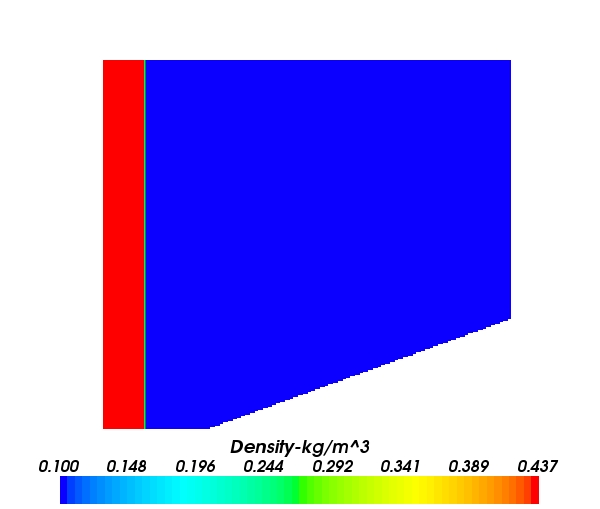
\includegraphics[width=5cm]{pics/cone_eg/cone0.jpg}
	}
	\subfigure[Density contours at 0.5 ms]{
	  \label{fig:cone20_r_us1}
	  \includegraphics[width=5cm]{../../paper_axisym_2006/pics/cone64-1_5.jpg}
	}
	\subfigure[Steady-state result] {
	  \label{fig:cone20_r_s1}
	  \includegraphics[width=5cm]{../../paper_axisym_2006/pics/cone64-1_5_final.jpg}
	}
	\caption{Density contours}
	\label{fig:VCE_20_deg_unsteady}
\end{figure}
\pagebreak

\section{Shock diffraction over blast wall}\label{sec:smith_barrier}

This test case attempts to duplicate Chapman's \cite{Chapman:bw} axisymmetric simulation of a blast wave propagating over a blast wall or
barrier.  The charge of 60 g of TNT is detonated at a 0.15 m height, 1.05 m from the the target structure (behind the blast wall) where
the pressure trace at 0.15 m height will be recorded (see the initial grid in fig~\ref{fig:grid_smith1}).  In this
simulation the domain is identically 1.05 m in length.  This size should be sufficient to produce the main rise and decay of 
the overpressure before effects from the non-reflecting boundary affect the solution.

The geometry and input files are in \verb'Octvce3.5.'$\star$\verb'/tests/smith_barrier_eg/'.

\subsection{Blast barrier geometry}\label{sec:smith_geom}

As this is an axisymmetric simulation, the geometry must be constructed in the manner described in $\mathsection$\ref{sec:2D}.
As the $x$ axis is the axis of symmetry (in this case the height) and $y$ the radial co-ordinate, the whole geometry must be 
constructed such that the \emph{west} boundary at $x = 0$ is the true `ground'.

A number of the geometry files have names corresponding to those of cone simulation ($\mathsection$\ref{sec:cone_geom}) and their
function is similar.  The file \verb'back_wall.vtp' corresponds to the true `ground' (preventing flow out the west boundary).
Note the slight overlap in geometry and domain as discussed in $\mathsection$\ref{sec:grid_flush} and $\mathsection$\ref{sec:cone_geom}.
The whole geometry is displayed in fig~\ref{fig:smith_geomfig}.

\begin{figure}[htp]
\centering
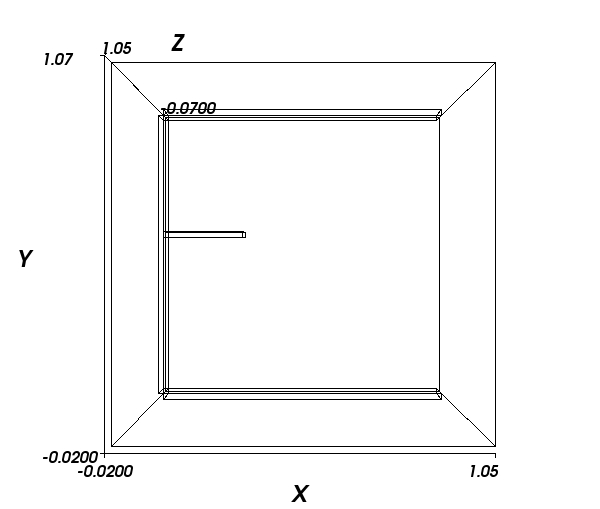
\includegraphics[width=6.5cm]{pics/smith_barrier_eg/sgeom.jpg}
\caption{Geometry for blast barrier simulation}
\label{fig:smith_geomfig}
\end{figure}

\subsection{Input files for blast barrier simulation}\label{sec:smith_par}

All input files are located in \verb'Octvce3.5'$\star$\verb'/tests/smith_barrier_eg/*.par'.

\subsubsection{General simulation parameters file}

This file has been called \verb'ov.par'.

\subsubsection{IC input file}

This file is called \verb'ov_IC.par'.

As this is a high explosives simulation the initial condition for the explosive products has been initalized in the manner described
in $\mathsection$\ref{sec:explo}, using Lee's JWL values for TNT \cite{Lee:ae}.  The geometry file for the spherical charge is
\verb'sphere.vtp' (centered at $x = 0.15$ m, $y = 0$).  Because of the axisymmetry, the actual bomb volume is a semi-circle.  

\subsubsection{Gas model input file}

This file is called \verb'ov_gas.par'.  2 species are necessary for the ambient and explosive products gases.  The JWL values
from Lee's paper \cite{Lee:ae} for TNT have been entered (in SI units).

\subsubsection{Domain BC input file}

This file is called \verb'ov_BC.par'.  It is identical to the one in fig~\ref{fig:ov_BC.par} as non-reflecting conditions
need to be placed on all boundaries (where they aren't blocked by walls).

\subsection{Running the blast barrier simulation}\label{sec:smith_run}

Before running the simulation it is important to count the total blast energy to ensure it matches the theoretical value
as close as possible (recall the discussion in $\mathsection$\ref{sec:explo}).  If the charge consisted of solid TNT then using 
according to the JWL parameters it would have a 
radius of $2.0636 \times 10^{-2}$ m and the energy for 60 g would be $4.1 \times 10^4$ J/rad (for a semi-circle).  So the code is run 
and the output shown in fig~\ref{fig:smith_counte}.   

\begin{figure}[htp]
\centering
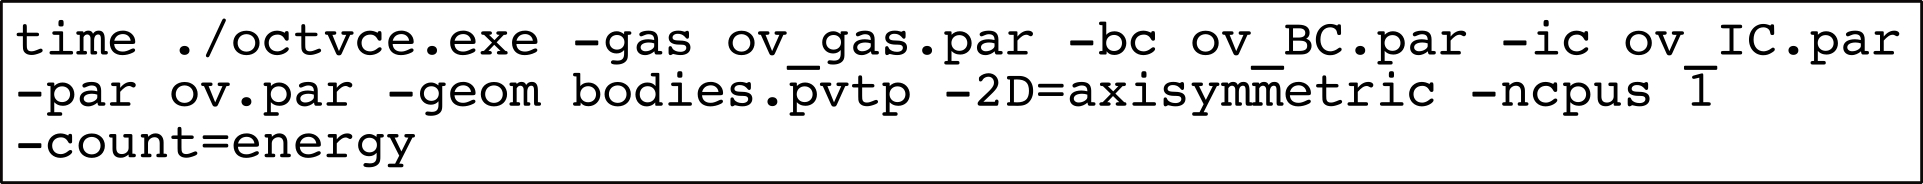
\includegraphics[width=14cm]{pics/cmd_exe_barrier1.jpg}
\caption{Running the blast barrier simulation}
\label{fig:smith_run}
\end{figure}

\begin{figure}[htp]
\centering
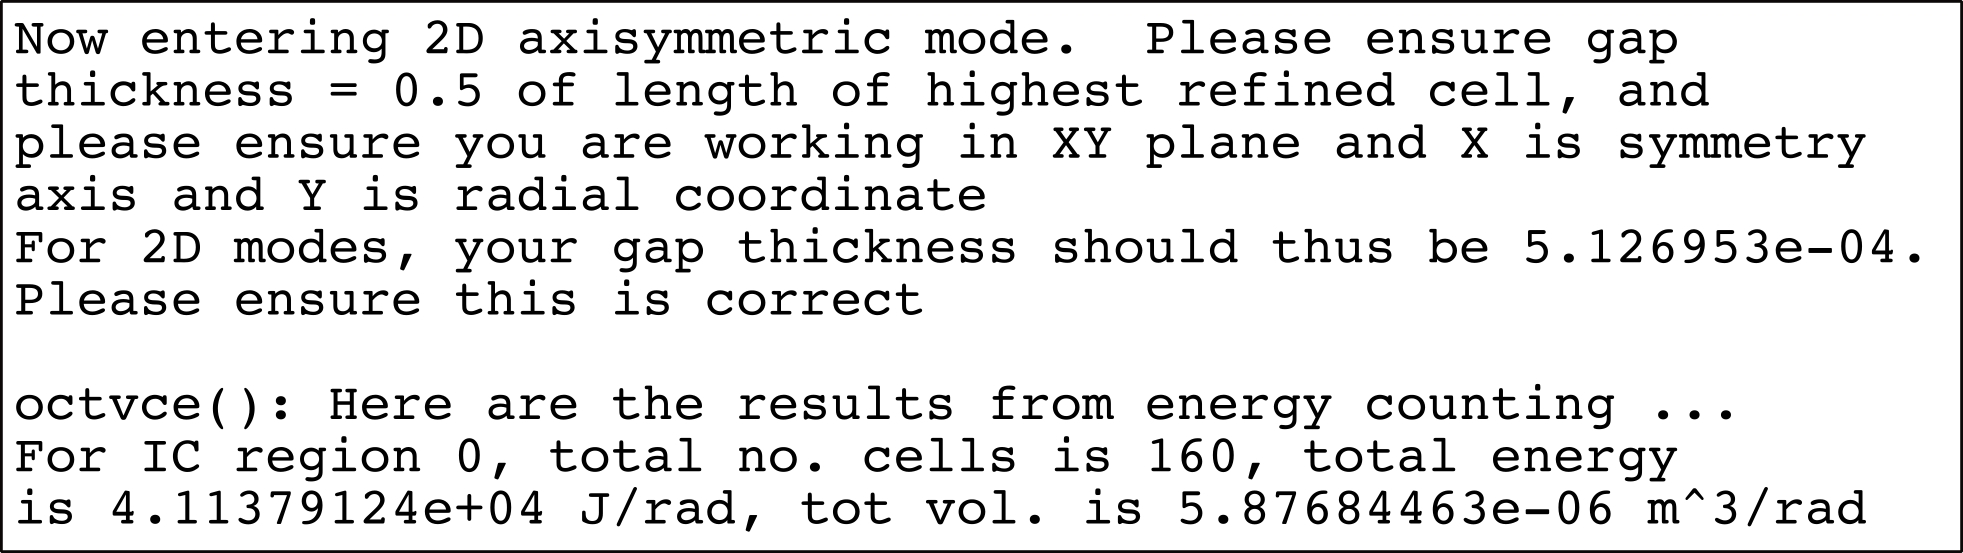
\includegraphics[width=13cm]{pics/barrier_output.jpg}
\caption{Energy counting results for blast wall simulation}
\label{fig:smith_counte}
\end{figure}

The energy count gives $4.114 \times 10^4$ J/rad (there were 160 cells representing the bomb volume).  The sphere radius used 
in \verb'sphere.vtp' was $2.018 \times 10^{-2}$ m, which is slightly smaller than theoretical whilst preserving the same shape.
As discussed in $\mathsection$\ref{sec:IC_advice} it is possible to use the total volume of cells within the bomb (here it is
$5.877 \times 10^{-6}$ m$^\text{3}$/rad) to adjust the initial bomb condition for an exact energy match, but this strategy isn't implemented here.
When one is satisfied with the energy match, the code can be run without the \verb'-count=energy' argument. 

\subsection{Some results for blast wall simulation}\label{sec:smith_results}

The initial grid is seen in fig~\ref{fig:grid_smith0} (the figure has been inverted so that the ground is at the `bottom').
The density contours and grid at 1 ms are shown in figs~\ref{fig:rcont_smith1} and~\ref{fig:grid_smith1}.  Note in
fig~\ref{fig:rcont_smith2} that at 2 ms the primary shock has exited the domain, but no reflections exist because of the non-reflecting boundary condition.  The
pressure trace at the gauge location is shown in fig~\ref{fig:ptrace_smith} and compared to Chapman's values.

\begin{figure}[htp]
  	\centering
	\subfigure[Initial grid]{
	  \label{fig:grid_smith0}
	  \includegraphics[width=5.9cm]{../../Simulation_pics/smith_grid0.jpg}
	}
	\subfigure[Density contours at 1 ms]{
	  \label{fig:rcont_smith1}
	  \includegraphics[width=5.9cm]{../../Simulation_pics/smith_r_cont1.jpg}
	}
	\subfigure[Grid and schlieren at 1 ms]{
	  \label{fig:grid_smith1}
	  \includegraphics[width=5.9cm]{../../Simulation_pics/smith_grid1.jpg}
	}
	\subfigure[Density contours at 2 ms]{
	  \label{fig:rcont_smith2}
	  \includegraphics[width=5.9cm]{../../Simulation_pics/smith_r_cont2b_nonreflect.jpg}
	}
	\subfigure[Pressure trace]{
	  \label{fig:ptrace_smith}
	  \includegraphics[width=9cm]{../../Simulation_pics/Smith_barrier.jpg}
	}
	\caption{Blast wall results}
	\label{fig:smith_wall_results}
\end{figure}

\pagebreak

\section{Blast over 3D obstructions}\label{sec:Rigas}

This 3D test case attempts to duplicate Sklavounos' investigation \cite{Rigas:cs} on blast wave effects with concrete blocks.
Sklavounos appears to model the blast using a finite energy
release rate which releases a total energy of $1.908 \times 10^6$ J, or 444 g TNT equivalent. This simulation takes advantage of 
the symmetry plane through the center of the blocks.  This simulation was terminated before any waves passed out of the domain.
A root cell length of 10 m was used (this should be enough before any boundary effects to intefere the trace readings).

The geometry and input files are in \verb'Octvce3.5.'$\star$\verb'/tests/rigas_eg/'.

\subsection{Obstruction geometries}\label{sec:Rigas_geom}

Explanation on the nature of some VTK files is necessary.
As the explosion takes place at the lower left corner of the domain, the file \verb'right_wall.vtp' places a wall at $y = 0$
to give the symmetry plane throught the center of the blocks.  However the file \verb'back_wall.vtp' also places a
symmetry plane at $x = 0$ to save computation time (the reflection from this boundary won't affect the initial gauge overpressure
readings).

The \verb'ceiling.vtp' and \verb'left_blocker.vtp' files reduce the domain size along the $y$ and $z$ axes as 
reflections from them will arrive far too late to affect initial gauge readings.  However the domain length along the
$x$ axis is kept at 10 m and a non-reflection boundary condition is active at the east face of the root cell.

\subsection{Input files for 3D obstruction simulation}\label{sec:Rigas_par}

The input files are in \verb'Octvce3.5'$\star$\verb'/tests/rigas_eg/*.par'.  

\subsubsection{General simulation parameters file}

This file is called \verb'ov.par'.

Note that adaptation indicator type 3 is used (which is just indicators 1 and 2 used together).  From 
$\mathsection$\ref{sec:ov_par} it was recommended that indicator type 1 vary from 0.01 to 0.05, but here it is 0.005.  This
value was chosen as the domain is relatively large compared to the initial explosive, and particularly after the blast
diffracts over the obstacles an indicator value greater 0.005 won't refine any cells around the shock.  

\subsubsection{IC input file}

This file is called \verb'ov_IC.par'.
TNT has been used as the explosive, so this file is very similar to the one in $\mathsection$\ref{sec:smith_par}.
Note that because there are 2 symmetry planes and the assumption that the charge is at ground level, the bomb volume is actually
a quarter hemi-sphere (i.e.\ a sphere octant).  The theoretical energy in this volume should be $4.77 \times 10^5$ J, but
at the given resolution the best match is $5.215 \times 10^5$ J (with a smaller sphere radius).

\subsubsection{Gas model input file}

This file is called \verb'ov_gas.par'.  It is also exactly identical to gas model input file in $\mathsection$\ref{sec:smith_par}. 

\subsubsection{Domain BC input file}

This file is called \verb'ov_BC.par'.  It is also exactly identical to gas model input file in $\mathsection$\ref{sec:smith_par}.

\subsection{Running the 3D obstruction simulation}\label{sec:Rigas_run}

Recall $\mathsection$\ref{sec:smith_run} where the total energy and bomb volume are first counted in an attempt to match best the 
theoretical total energy.  Once an appropriate energy match is achieved the simulation is finally run (here it was using 8 threads) with
the command line arguments

\begin{figure}[htp]
\centering
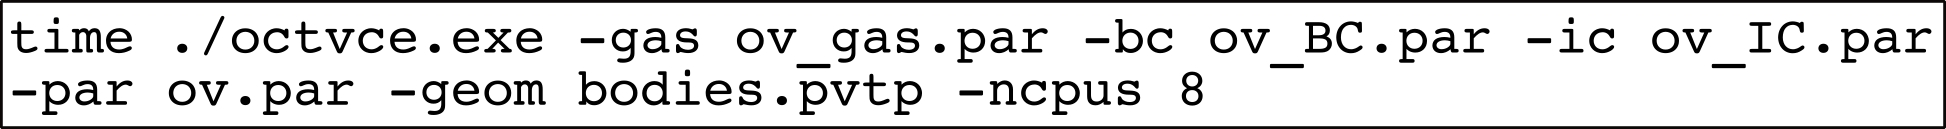
\includegraphics[width=13cm]{pics/cmd_exe_rigas.jpg}
\caption{Running the 3D obstruction simulation}
\label{fig:rigas_run}
\end{figure}

\subsection{Some results for 3D obstruction simulation}\label{sec:Rigas_results}

Fig~\ref{fig:rigas_trace1} shows the pressure trace at gauge 1 of Sklavounos' simulation (this gauge is positioned between the
first and second concrete blocks).  His computational and experimental results are also shown for comparison (they had to
be estimated by eye).  It can be seen that agreement is quite good with the expectd first three peaks being the incident shock and
the reflected shocks from the ground and the second concrete block.

Fig~\ref{fig:rigas_trace2} is the pressure trace at gauge 2 (between the second and third concrete blocks).  As with the gauge 1 
trace the agreement in peak overpressure and general waveform profile is good, although here the waveform is more complex given 
the reflections that have occured before the blast reached this gauge.  Fig~\ref{fig:rigas_rcont} shows the mesh and 
density contours on planes intersecting the blast centre.  

\begin{figure}[htp]
  	\centering
	\subfigure[Trace at gauge 1]{
	  \label{fig:rigas_trace1}
	  \includegraphics[width=9cm]{../../Simulation_pics/Rigas0b.jpg}
	}
	\subfigure[Trace at gauge 2]{
	  \label{fig:rigas_trace2}
	  \includegraphics[width=9cm]{../../Simulation_pics/Rigas1b.jpg}
	}
	\subfigure[Density contours]{
	  \label{fig:rigas_rcont}
	  \includegraphics[width=7.5cm]{../../paper_2006/pics/Rigas_r_cont.jpg}
	}
	\caption{3D obstruction results}
	\label{fig:rigas_results}
\end{figure}

\addcontentsline{toc}{chapter}{Bibliography}
\bibliography{../../Biblio/bib_so_far}
\end{document}
